\documentclass[12pt]{article}
\usepackage[brazil]{babel}
\usepackage{setspace}
\usepackage{boxedminipage}
\usepackage[latin1]{inputenc}
\usepackage{latexsym}
\usepackage{amsfonts}
\usepackage{hyperref}
\usepackage{graphicx}
\usepackage{wrapfig}
\usepackage{longtable}
\usepackage{subfigure}
\usepackage{epsfig}
\usepackage[font=small, textfont=it, labelfont=bf]{caption}
\usepackage{caption}
\usepackage{listings}
\usepackage{color}

\setlength{\paperheight}{29.7cm}
\setlength{\footskip}{1.0cm}
\setlength{\textheight}{20.0cm}
\setlength{\textwidth}{16.0cm}
\setlength{\oddsidemargin}{0.0cm}
\setlength{\topmargin}{0.0cm}

\definecolor{lbcolor}{rgb}{0.9,0.9,0.9}
\lstset{backgroundcolor=\color{lbcolor},rulecolor=}
\lstset{language=C++}
\lstset{basicstyle=\footnotesize}

\lstnewenvironment{codigo}
{\lstset{frame=single}}
{}

\begin{document}
\title{Pandora's Box Graphic Engine - Uma Engine Gr�fica com Aplica��o em Visualiza��o de Campos Tensoriais}
\author{Andrew Toshiaki Nakayama Kurauchi \and Victor Kendy Harada \\ Orientador: Prof. Dr. Marcel Parolin Jackowski}
\maketitle
\thispagestyle{empty}

\newpage
\setcounter{page}{1}
\tableofcontents

\section{Introdu��o}
%Apresenta��o de engines gr�ficas alternativas existentes e os motivos para a cria��o de mais uma alternativa. Import�ncia da visualiza��o de campos tensoriais e como uma engine gr�fica pode auxiliar o desenvolvimento de aplica��es com tal prop�sito.
	O desenvolvimento de programas de computa��o gr�fica em tempo real exige a aplica��o de um vasto conjunto de t�cnicas de otimiza��o que s�o recorrentes em diversos aplicativos. Por esse motivo s�o desenvolvidas engines gr�ficas como OpenSceneGraph~\cite{openscenegraph} e Ogre3D~\cite{ogre3d}. Entretanto, tais engines evolu�ram de tal forma que o tempo de aprendizagem � longo. O intuito desse trabalho � desenvolver uma engine gr�fica que implemente t�cnicas b�sicas de computa��o gr�fica e que seja f�cil de ser aprendida e utilizada.

	O estudo de tensores e campos tensoriais � de import�ncia fundamental para diversas �reas do conhecimento. S�o encontradas aplica��es no estudo de fen�menos s�smicos~\cite{Engelsma_cwp-655visualization}, estruturas eletr�nicas~\cite{electronic-structure} e imagens de resson�ncia magn�tica sens�veis a difus�o~\cite{citeulike:3787472}. A visualiza��o de tais campos �, portanto, de grande relev�ncia para o avan�o do conhecimento. Por esse motivo uma das aplica��es desenvolvidas com o aux�lio da engine ser� um programa que permita tais visualiza��es. Ser�o utilizados para testes a visualiza��o da representa��o elipsoidal de campos tensoriais provenientes de imagens de resson�ncia magn�tica sens�veis a difus�o e campos representativos de deforma��es f�sicas em 3 dimens�es.


\section{Conceitos e tecnologias estudadas}
A seguir ser�o apresentados os conceitos e tecnologias utilizadas na implementa��o da engine, assim como na aplica��o de exemplo (visualiza��o de campos tensoriais).

\subsection{Linguagem C++98}
A linguagem de programa��o C++ foi desenvolvida como uma evolu��o da linguagem C. Por esse motivo a sintaxe de ambas � semelhante e um c�digo escrito em C � v�lido em C++. � uma linguagem estruturada que, entre outras caracter�sticas, adiciona o paradigma de orienta��o a objetos ao C.

\subsubsection{Vari�veis e fun��es}
As vari�veis e fun��es s�o declaradas com a mesma sintaxe utilizada na linguagem C (um qualificador seguido de um tipo e de um nome, podendo receber um valor inicial):

% Pensar em uma forma melhor de mostrar isso.
\begin{verbatim}
<qualificador> <tipo> <nome>[=<valor inicial>]
\end{verbatim}

\subsubsection{Classes e objetos}
Classes s�o definidas pelas palavras reservadas \texttt{class} ou \texttt{struct}, sendo que a diferen�a entre elas � o fato de atributos de uma \texttt{class} serem privados por padr�o e os de uma \texttt{struct}, p�blicos. � poss�vel adicionar modificadores de acesso atrav�s das palavras \texttt{public}, \texttt{private} e \texttt{protected} que definem acesso livre em todos os escopos, acesso restrito � classe e acesso restrito � classe e suas subclasses respectivamente. Construtores s�o declarados como fun��es com o nome da classe. A declara��o de uma classe \texttt{Coordenada2d} poderia ocorrer das seguintes maneiras:

Utilizando \texttt{class}:

\begin{verbatim}
class Coordenada2d {
public:
    Coordenada2d(double x, double y);
private:
    double x,y;
};
\end{verbatim}

Utilizando \texttt{struct}:

\begin{verbatim}
struct Coordenada2d {
    double x,y;
};
\end{verbatim}

Para se instanciar um objeto existem duas op��es. A primeira consiste em declarar uma vari�vel da classe desejada (da mesma forma como vari�veis do tipo \texttt{int} s�o declaradas, por exemplo). Na declara��o da vari�vel a classe ser� instanciada e inicializada. A segunda maneira � a utiliza��o da palavra reservada \texttt{new} seguida do nome da classe. O valor devolvido � um ponteiro para uma inst�ncia da classe desejada. Seguindo o exemplo anterior, a classe Coordenada2d poderia ser instanciada das seguintes formas:

\begin{verbatim}
Coordenada2d coordenada1;
Coordenada2d * coordenada2 = new Coordenada2d;
\end{verbatim}

Os argumentos do construtor s�o passados da seguinte maneira:

\begin{verbatim}
Coordenada2d coordenada1(1.0, 2.0);
Coordenada2d * coordenada2 = new Coordenada2d(1.0, 2.0);
\end{verbatim}

\subsubsection{Namespaces}
Para evitar colis�o de identificadores como nomes de classes, vari�veis e fun��es � poss�vel utilizar um \texttt{namespace}:

\begin{verbatim}
namespace nome {
// Entidades
    int n;
}
\end{verbatim}

Onde \texttt{nome} � qualquer identificador v�lido e \texttt{Entidades} � o conjunto de classes, vari�veis e fun��es que ficar�o protegidas dentro de um \texttt{namespace}.

Para referenciar identificadores de um \texttt{namespace} � utilizada a seguinte sintaxe:

\begin{verbatim}
<nome do namespace>::<identificador>
\end{verbatim}

Para acessar a vari�vel \texttt{n} do exemplo utiliza-se o seguinte c�digo:

\begin{verbatim}
nome::n
\end{verbatim}

\subsubsection{Templates}
O template � um recurso da linguagem C++ que permite programa��o gen�rica. � utilizado para a implementa��o de fun��es ou classes cujas funcionalidades podem ser adaptadas para tipos diferentes com o mesmo c�digo. Para isso � utilizada a palavra reservada \texttt{template} seguida por um par�metro de template, que � um tipo especial de par�metro que pode ser utilizado para enviar tipos como argumento.

Uma fun��o \texttt{maximo} poderia ser definida da seguinte maneira:

\begin{verbatim}
template <class T>
T maximo(T a, T b) {
    T resultado;
    resultado = (a > b) ? a : b;
    return resultado;
}
\end{verbatim}

Para utiliz�-la deve ser enviado o tipo dos argumentos utilizados:

\begin{verbatim}
int c = 4, d = 5;
maximo<int>(c,d);
\end{verbatim}

Um n� de uma lista ligada gen�rica poderia ser implementado de maneira an�loga:

\begin{verbatim}
template <class T>
class No {
public:
    No(T valorInicial) {
        valor = valorInicial;
        proximo = NULL;
    }
    T getValor() {
        return valor;
    }
    void setValor(T novoValor) {
        valor = novoValor;
    }
    No<T> * getProximo() {
        return proximo;
    }
    void setProximo(No<T> *novoProximo) {
        proximo = novoProximo;
    }
private:
    T valor;
    No<T> *proximo;
};
\end{verbatim}

A utiliza��o tamb�m � an�loga � de fun��es:

\begin{verbatim}
No<int> meuNo(5);
\end{verbatim}

\subsubsection{A Standard Template Library (STL)}

A Standard Template Library (STL)~\cite{stl}� uma biblioteca C++ baseada em templates que oferece um conjunto de algoritmos e estruturas de dados configur�veis.

� poss�vel, por exemplo, aplicar uma fun��o para todos os itens de um vetor de inteiros da seguinte maneira:

\begin{verbatim}
void imprime(int i) {
    printf("%d ", i);
}

int main() {
    std::vector<int> vetor;
    // Adicionando os valores 1, 2 e 3 no vetor
    vetor.push_back(1);
    vetor.push_back(2);
    vetor.push_back(3);

    for_each(vetor.begin(), vetor.end(), imprime);
    // Sa�da: 1 2 3

    return 0;
}
\end{verbatim}

O m�todo \texttt{for\_each} pode, alternativamente, receber um objeto com a fun��o a ser aplicada a cada item da lista definida na sobrescrita do operador \texttt{()} como a seguir:

\begin{verbatim}
struct impressor {
    void operator() (int i) {
        printf("%d ", i);
    }
} meuImpressor;

int main() {
    std::vector<int> vetor;
    vetor.push_back(1);
    vetor.push_back(2);
    vetor.push_back(3);

    for_each(vetor.begin(), vetor.end(), meuImpressor);
    // Sa�da: 1 2 3

    return 0;
}
\end{verbatim}

H� diversos outros tipos de algoritmos implementados na STL~\cite{algorithm}

\subsection{Boost C++ Libraries}

Boost~\cite{boost} � uma biblioteca de C++ de c�digo aberto inicialmente desenvolvida como uma extens�o para a STL sob o namespace \texttt{boost}. Os principais m�dulos dessa biblioteca utilizados no desenvolvimento da engine foram \texttt{bind}, \texttt{function} e \texttt{smart\_ptr}. 

O m�dulo \texttt{function} cria functors (objetos de fun��o) que s�o capazes de armazenar tanto fun��es nativas da linguagem quanto outros functors. Essas fun��es s�o criadas atrav�s da seguinte constru��o:

\begin{verbatim}
void f (int i, int j, int k) {
    // implementa��o
}
// boost::function[numero de argumentos]<tipo de retorno, tipos dos argumentos>
boost::function3<void,int,int,int> funcao = f;
\end{verbatim}

A biblioteca \texttt{bind} cria functors (classes que implementam o m�todo \texttt{operator ()}) a partir de uma fun��o ou outro functor mas com alguns argumentos j� posicionados, por exemplo:

\begin{verbatim}
boost::bind(f, 1, _1, _2)
\end{verbatim}

Nesse caso boost::bind cria um functor que recebe apenas dois argumentos, indicados pelos nomes \_1 e \_2, o primeiro e o segundo argumento do functor criado respectivamente.

As funcionalidades de bind e function podem ser combinadas:

\begin{verbatim}
// functor sem retorno que recebe dois argumentos inteiros
boost::function2<void, int, int> functor1 = boost::bind(f, 1, _1, _2);
// cria um boost::function a partir do resultado do boost::bind de uma 
// boost::function
boost::function1<void, int> functor2 = boost::bind(functor1, 2, _1);
\end{verbatim}

Os m�dulos bind e function da boost s�o utilizados principalmente em conjunto com algoritmos da STL, como o std::for\_each. %TODO: exemplo de c�digo?

Os \texttt{smart\_ptr} s�o classes que guardam ponteiros para �reas de mem�ria alocadas dinamicamente. Essas classes tem comportamento parecido com o de ponteiros nativos da linguagem, com a diferen�a de que elas desalocam o recurso a que referenciam em momento adequado. Existem seis tipos \texttt{smart\_ptr} definidos:

\begin{itemize}
\item \texttt{scoped\_ptr}: representa o conceito de ponteiro n�o compartilh�vel, logo n�o podem ser copiados. Desalocam a mem�ria ao sair de escopo.
\item \texttt{scoped\_array}: mesmo que \texttt{scoped\_ptr} mas para um array de objetos.
\item \texttt{shared\_ptr}: representa um ponteiro que tem diversos donos, pode ser copiado e s� � destru�do quando todos os donos forem destru�dos.
\item \texttt{shared\_array}: mesmo que \texttt{shared\_ptr} mas para arrays.
\item \texttt{weak\_ptr}: s�o ponteiros para recursos de um \texttt{shared\_ptr} mas que n�o s�o donos do recurso.
\item \texttt{intrusive\_ptr}: s�o \texttt{shared\_ptr} que guardam dentro do objeto para o qual apontam o contador de refer�ncias utilizado internamente.
\end{itemize}

\subsection{OpenGL}

O OpenGL � uma especifica��o aberta e extens�vel de uma interface de software para o hardware gr�fico.

%todo: falar sobre a extensibilidade � importante!!!

\subsubsection{O que ele n�o faz}

O OpenGL n�o realiza tratamentos que dependam do sistema operacional, ou seja, n�o gerencia janelas, nem controla eventos de entrada e sa�da.

Al�m disso ele n�o disponibiliza nenhuma forma de leitura de arquivos. Por esse motivo, n�o � poss�vel visualizar diretamente imagens guardadas em arquivos (como png, jpg, bmp, ou modelos em tr�s dimens�es como 3ds\cite{3dsfileformat}, blend\cite{blendfileformat}, ou obj\cite{objfileformat}).

\subsubsection{O que ele faz}

O OpenGL � capaz de representar v�rtices em tr�s dimens�es combinados em pontos, retas, tri�ngulos e quadril�teros, chamados de primitivas.

Tais primitivas s�o projetadas em um plano e transformadas em conjuntos de pixels. Essa transforma��o, conhecida como rasteriza��o � parte do processo descrito a seguir.

\subsection{O pipeline}

As primitivas geradas na CPU (Central Processing Unit) s�o enviadas para a GPU (Graphics Processing Unit) onde ser�o processadas e utilizadas para gerar uma imagem que ser� mostrada na janela. %TODO Explicar cada parte, falar o que s�o shaders e depois falar o nome Pipeline 

\includegraphics{pipeline}

\subsection{GLEW}

A \texttt{OpenGL Extension Wrangler Library}  \cite{glew}, conhecida como \texttt{GLEW} � uma biblioteca que auxilia no gerenciamento de extens�es do OpenGL. Ela � capaz de obter as fun��es definidas por extens�es do OpenGL e al�m disso, fornece constantes definidas em tempo de execu��o que cont�m as extens�es do OpenGL que o sistema do usu�rio suporta.

O uso da \texttt{GLEW} � ilustrado no c�digo abaixo:

\begin{verbatim}
#include <GL/glew.h>
// Ap�s a inicializa��o do contexto do OpenGL
glewInit();
// ap�s a inicializa��o as fun��es definidas atrav�s de extens�es est�o dispon�veis

// verificar se a extens�o GL_ARB_vertex_program est� dispon�vel
if(GLEW_ARB_vertex_program) {
    ...
}
// ou
if(glewIsSupported("GL_ARB_vertex_program")) {

}
\end{verbatim}

\subsection{Windows API}
Como citado anteriormente, o OpenGL n�o � respons�vel por criar janelas e tratar eventos gerados pelo sistema operacional, esse tratamento � dependente do ambiente no qual o programa ser� executado. Nesse trabalho foi utilizada apenas a API do sistema operacional Windows.

%TODO: N�o esquecer de explicar a ideia do contexto na parte de OpenGL
Para se inicializar um contexto para a execu��o de programas em OpenGL � necess�rio criar uma janela, para isso usa-se a seguinte fun��o\cite{doccreatewindow}:

\begin{verbatim}
HWND WINAPI CreateWindow(
  __in_opt  LPCTSTR lpClassName,
  __in_opt  LPCTSTR lpWindowName,
  __in      DWORD dwStyle,
  __in      int x,
  __in      int y,
  __in      int nWidth,
  __in      int nHeight,
  __in_opt  HWND hWndParent,
  __in_opt  HMENU hMenu,
  __in_opt  HINSTANCE hInstance,
  __in_opt  LPVOID lpParam
);
\end{verbatim}

Onde:
\begin{itemize}
\item \texttt{lpClassName}: representa uma classe registrada anteriormente no sistema.
\item \texttt{lpWindowName}: representa o t�tulo da janela.
\item \texttt{dwStyle}: conjunto de flags que definem como a janela ser� exibida\cite{docwindowstyle}: com bordas, maximizada, minimizada, \ldots
\item \texttt{x, y}: posi��o inicial da janela.
\item \texttt{nWidth, nHeight}: dimens�es iniciais da janela.
\item \texttt{hWndParent}: se a janela que est� sendo criada � uma subjanela de uma j� existente, passa-se o handler da janela pai nesse argumento, caso contr�rio, passa-se \texttt{NULL}. Para a engine gr�fica, esse argumento sempre recebe o valor \texttt{NULL}.
\item \texttt{hMenu}: se for necess�rio criar uma menu, deve-se passar o handler do menu nesse argumento, caso contr�rio, passa-se \texttt{NULL}. %Falar o que � um handler
\item \texttt{hInstance}: o handler da inst�ncia do programa que est� sendo executado, esse par�metro � utilizado dentro do sistema na cria��o de um identificador �nico para a janela.
\item \texttt{lpParam}: dados do usu�rio. Esse par�metro recebe um ponteiro para qualquer tipo de dado que o usu�rio necessite. Na engine esse argumento recebe o ponteiro para uma inst�ncia de uma classe interna que representa a janela do sistema.
\end{itemize}

Para se registrar uma classe no sistema deve-se chamar a fun��o\cite{docregisterclass}:
\begin{verbatim}
ATOM WINAPI RegisterClass(
  __in  const WNDCLASS *lpWndClass
);
\end{verbatim}

O argumento \texttt{lpWndClass} um ponteiro para uma inst�ncia de \texttt{WNDCLASS}\cite{docwndclass}, uma estrutura que guarda, entre outras coisas, o nome da classe que est� sendo registrada, o ponteiro para a fun��o que ir� tratar os eventos gerados pelo sistema e uma flag que indica se o contexto do dispositivo\cite{docdevicecontext} pode ser compartilhado. Quando se cria um contexto do OpenGL � importante sempre registrar a classe como dona do contexto do dispositivo. %TODO: Por que isso?

Ap�s criada, deve-se avisar o sistema que a janela � vis�vel, para isso, executa-se\cite{docshowwindow}:

\begin{verbatim}
BOOL WINAPI ShowWindow(
  __in  HWND hWnd,
  __in  int nCmdShow
);
\end{verbatim}

%TODO: Explicar em algum lugar o que s�o handlers (por mais simples que isso soe)
Onde \texttt{hWnd} � o handler devolvido pela fun��o \texttt{CreateWindow} e \texttt{nCmdShow} controla como a janela deve ser exibida (maximizada, minimizada, simplesmente exibida, \ldots)

% TODO: Em nenhum lugar foi citado que o trabalho � dividido em threads
Depois de criar a janela, a thread m�e come�a a receber os eventos da janela criada em sua fila de mensagens. Para se recuperar uma mensagem da fila, utiliza-se a fun��o\cite{docgetmessage}:

\begin{verbatim}
BOOL WINAPI GetMessage(
  __out     LPMSG lpMsg,
  __in_opt  HWND hWnd,
  __in      UINT wMsgFilterMin,
  __in      UINT wMsgFilterMax
);
\end{verbatim}

Que recebe como par�metros um ponteiro para uma estrutura do tipo \texttt{MSG}\cite{docmsg}, o handler devolvido pela fun��o \texttt{CreateWindow}, \texttt{wMsgFilterMin} e \texttt{wMsgFilterMax} s�o constantes que podem ser passadas para indicar que tipo de mensagem deve ser retornada. O valor de retorno dessa fun��o � um inteiro que indica qual o tipo de mensagem foi retornada ou se ocorreu um erro durante a execu��o da fun��o.

Ap�s recuperar a mensagem ela precisa ser traduzida e em seguida enviada para o seu destino final, a fun��o respons�vel pela tradu��o da mensagem �\cite{doctranslatemessage}

\begin{verbatim}
BOOL WINAPI TranslateMessage(
  __in  const MSG *lpMsg
);
\end{verbatim}

e a fun��o que envia a mensagem para a janela �\cite{docdispatchmessage}:

\begin{verbatim}
LRESULT WINAPI DispatchMessage(
  __in  const MSG *lpmsg
);
\end{verbatim}

Quando a thread principal recebe a mensagem \texttt{WM\_QUIT}, o retorno de \texttt{GetMessage} � \texttt{0}, nesse momento a tradu��o e envio de mensagens deve parar e o programa deve apagar o registro da classe criada por \texttt{RegisterClass}. O registro � apagado pela fun��o\cite{docunregisterclass}:

\begin{verbatim}
BOOL WINAPI UnregisterClass(
  __in      LPCTSTR lpClassName,
  __in_opt  HINSTANCE hInstance
);
\end{verbatim}

que recebe como argumentos o nome com o qual a classe foi registrada e a inst�ncia do programa que registrou a classe.

\subsubsection{O loop de eventos da janela}

A fun��o registrada na WNDCLASS que tratar� os eventos gerados pelo sistema deve ter a seguinte assinatura\cite{docwindowproc}:
\begin{verbatim}
LRESULT CALLBACK WindowProc(
  __in  HWND hwnd,
  __in  UINT uMsg,
  __in  WPARAM wParam,
  __in  LPARAM lParam
);
\end{verbatim}

Nessa fun��o, o argumento hwnd � o handler da janela corrente, uMsg � um inteiro sem sinal que c�difica a mensagem recebida e os argumentos wParam e lParam s�o os par�metros da mensagem.

Por exemplo:
% falar sobre window resize...

Um la�o de eventos t�pico para um programa em OpenGL tem a seguinte forma:

\begin{verbatim}
LRESULT CALLBACK WindowProc(HWND hWnd, UINT msg, WPARAM wParam, LPARAM lParam){
	switch(msg) {
		case WM_CREATE: 
			// Inicializa��o do contexto de renderiza��o
			// no caso da WM_CREATE o valor de lParam � um ponteiro para um struct
			// do tipo CREATESTRUCT que cont�m o ponteiro para os dados do usu�rio
			// passado na fun��o CreateWindow
			
		case WM_DESTROY:
			// Libera��o de recursos gr�ficos e dele��o do contexto criado
		case WM_CLOSE:
			// O usu�rio clicou no bot�o de fechamento da janela
			// Ent�o deve-se avisar para o sistema operacional que a aplica��o deve
			// ser encerrada.
			PostQuitMessage(0);
			break;
		case WM_PAINT:
			// O sistema requisitou � aplica��o a atualiza��o da janela

			// Fun��es do OpenGL para limpar e renderizar
			wglSwapBuffers();
			// avisa ao sistema que o evento j� foi completamente tratado
			return 0;
	}
	// Executa a rotina padr�o para tratar o evento gerado
	return (DefWindowProc(hwnd, msg, wParam, lParam));
}
\end{verbatim}

Ao receber \texttt{WM\_CREATE} a aplica��o deve inicializar todos os recursos para que a janela possa ser utilizada. No caso da Pandora's Box utilizando OpenGL como API gr�fica, deve-se inicializar o contexto de renderiza��o que ser� utilizado.

% antes de chamarmos wglCreateContext devemos criar o pixel format descriptor
A cria��o do contexto � gerenciada pela API do wgl (tamb�m conhecido como Wiggle), que � a implementa��o de OpenGL para o Windows. O contexto que ser� utilizado pela aplica��o deve ser criado atrav�s da fun��o wglCreateContext \cite{wglcreatecontextdoc}: %TODO essa cita��o est� como [?]

\begin{verbatim}
% assinatura da wglCreateContext
\end{verbatim}

Essa fun��o tem como argumento o handler para o dispositivo utilizado pela janela. Tal handler pode ser obtido atrav�s da fun��o GetDC \cite{getdcdoc}: %TODO essa cita��o est� como [?]

% outro prototipo

Logo a cria��o do contexto pode ser feita pelo seguinte trecho de c�digo:

\begin{verbatim}
case WM_CREATE:
	HDC hDC = GetDC(hWnd);
	setPixelFormatDescriptor();
	HGLRC hglrc = wglCreateContext(hDC);
	wglMakeCurrent(hglrc);
	break;
\end{verbatim}

\subsection{Carregamento din�mico de dll}

Para que seja poss�vel suportar diversas implementa��es independentes de especifica��es de APIs gr�ficas, a engine possui um mecanismo de carregamento din�mico de dlls.

Para se executar c�digo presente em uma dll, � necess�rio carreg�-la durante a execu��o do programa. Atrav�s da windows API, pode-se abrir um arquivo dll com a fun��o LoadLibrary:

\begin{verbatim}
% prot�tipo da load library
\end{verbatim}

essa fun��o retorna o handler para a biblioteca carregada ou NULL caso tenha ocorrido um erro. Caso o carregamento seja bem sucedido, pode-se utilizar o handler obtido para procurar ponteiro de fun��es.

Na windows API, a fun��o que cuida da busca de ponteiros de fun��o � a GetProcAddress

\begin{verbatim}
% prot�tipo da get proc address
\end{verbatim}

essa fun��o devolve um ponteiro gen�rico do tipo void* que precisa ser transformado para um ponteiro de fun��o.

O carregamento de uma dll dynamic\_create.dll com uma fun��o chamada create � exemplificado no c�digo abaixo:

\begin{verbatim}
// fun��o que n�o recebe argumentos e retorna um ponteiro gen�rico
typedef void * (__cdecl * MYPROC)();

HINSTANCE lib = LoadLibrary(L"dynamic_create.dll");
MYPROC lib_create = (MYPROC)GetProcAddress(lib, L"create");
SomeObject object = (SomeObject) lib_create();
\end{verbatim}

Um detalhe importante do carregamento din�mico de bibliotecas escritas em C++, � que para permitir o uso de namespaces, classes e sobrecarga de fun��es, o compilador da linguagem muda os nomes das fun��es geradas. Logo se uma fun��o chamada create for compilada como um procedimento de c++, seu nome no arquivo dll n�o ser� create, mas sim um nome que depende da implementa��o do compilador utilizado. Para evitar a mudan�a de nomes, as fun��es a serem exportadas devem ser declaradas da forma abaixo:

\begin{verbatim}
extern "C" {
	// declara��o das fun��es a serem exportadas.
}
\end{verbatim}

Outro detalhe espec�fico do compilador da Microsoft, que foi utilizado nesse trabalho, � que os procedimentos que ser�o exportados devem ser definidos com a diretiva da seguinte forma:
\begin{verbatim}
__declspec(dllexport) TipoDeRetorno nome_da_funcao(parametros);
\end{verbatim}

\subsection{Transforma��es lineares}
O conceito de transforma��es lineares � de import�ncia fundamental para a computa��o gr�fica. Atrav�s delas � poss�vel representar transla��es, rota��es e escalas aplicadas sobre os objetos.

\subsubsection{Defini��o}
Sejam $U$ e $V$ espa�os vetoriais. Uma transforma��o linear � uma aplica��o~\cite{callioli2007algebra} $F: U \rightarrow V$, tal que:
\begin{enumerate}
\item $F(u_1 + u_2) = F(u_1) + F(u_2), \forall u_1, u_2 \in U$
\item $F(\alpha u) = \alpha F(u), \forall \alpha \in \mathbb{R}$ e $\forall u \in U$
\end{enumerate}

\subsubsection{Aplica��o em computa��o gr�fica}
Em computa��o gr�fica s�o utilizadas as coordenadas homog�neas~\cite{redbook} de v�rtices em $\mathbb{R}^3$. Para realizar a transla��o, rota��o e escala de objetos representados em tais coordenadas utiliza-se as seguintes matrizes de transforma��o linear:

Transla��o:

\begin{math}
\left(
\begin{array}{cccc}
1 & 0 & 0 & t_x \\
0 & 1 & 0 & t_y \\
0 & 0 & 1 & t_z \\
0 & 0 & 0 & 1 
\end{array}
\right)
\end{math}

Onde $t_x, t_y, t_z$ s�o as transla��es nos eixos $x, y, z$ respectivamente.

Rota��o no eixo x:

\begin{math}
\left(
\begin{array}{cccc}
1 & 0 & 0 & 0 \\
0 & cos\theta & -sen\theta & 0 \\
0 & sen\theta & cos\theta & 0 \\
0 & 0 & 0 & 1 
\end{array}
\right)
\end{math}

Rota��o no eixo y:

\begin{math}
\left(
\begin{array}{cccc}
cos\theta & 0 & sen\theta & 0 \\
0 & 1 & 0 & 0 \\
-sen\theta & 0 & cos\theta & 0 \\
0 & 0 & 0 & 1 
\end{array}
\right)
\end{math}

Rota��o no eixo z:

\begin{math}
\left(
\begin{array}{cccc}
cos\theta & -sen\theta & 0 & 0 \\
sen\theta & cos\theta & 0 & 0 \\
0 & 0 & 1 & 0 \\
0 & 0 & 0 & 1 
\end{array}
\right)
\end{math}

Onde $\theta$ � o �ngulo de rota��o.

Escala:

\begin{math}
\left(
\begin{array}{cccc}
s_x & 0 & 0 & 0 \\
0 & s_y & 0 & 0 \\
0 & 0 & s_z & 0 \\
0 & 0 & 0 & 1 
\end{array}
\right)
\end{math}

Onde $s_x, s_y, s_z$ s�o as escalas aplicadas nos eixos $x, y, z$ respectivamente.

As transforma��es podem ser compostas atrav�s de multiplica��es das matrizes.

\subsection{Tensores de imagens de resson�ncia magn�tica de difus�o}
Difus�o � o nome dado ao movimento aleat�rio de mol�culas em um fluido (l�quido ou gasoso). Denomina-se coeficiente de difus�o a facilidade com que uma mol�cula se move no meio. Em fluidos homog�neos, como a �gua, o coeficiente de difus�o � o mesmo em todas as dire��es. A esse tipo de meio d�-se o nome de isotr�pico. Em fluidos heterog�neos o coeficiente pode variar dependendo da dire��o. Esses s�o os meios anisotr�picos. Um exemplo de meio anisotr�pico s�o os tecidos biol�gicos.

Imagens de resson�ncia magn�tica de difus�o s�o uma das formas de obter informa��es sobre o coeficiente de difus�o de mol�culas de �gua em diferentes dire��es nesses tipos de tecidos.

Para representar tais coeficientes s�o utilizados tensores, que s�o abstra��es de escalares, vetores e matrizes utilizados em diversas aplica��es. Em imagens de resson�ncia magn�tica de difus�o, tais tensores s�o comumente representados por matrizes $ 3 \times 3 $ sim�tricas.

\subsection{Representa��o elipsoidal de tensores de difus�o}
Em meios isotr�picos o coeficiente de difus�o pode ser representado por uma esfera, pois o movimento das mol�culas se distribui igualmente para todas as dire��es em um determinado per�odo de tempo. J� em meios anisotr�picos, como o movimento depende da dire��o, o coeficiente � modelado como um elips�ide, sendo que os semi-eixos t�m comprimento proporcional aos autovalores do tensor ($\lambda_{1} > \lambda_{2} > \lambda_{3}$) ao longo dos seus autovetores $\epsilon_{1}, \epsilon_{2}, \epsilon_{3}$.

\subsection{Anisotropia Fracionada}
A anisotropia fracionada � um valor no intervalo $ [0,1] $ que descreve o grau de anisotropia de um processo de difus�o. Sejam $\lambda_{1}, \lambda_{2}, \lambda_{3}$ os autovalores do tensor. A anisotropia fracionada ($AF$) pode ser calculada a partir da seguinte f�rmula\cite{hagmann}:

\begin{equation}
AF = \sqrt{\frac{1}{2}}\frac{\sqrt{(\lambda_{1}-\lambda_{2})^{2} + (\lambda_{1}-\lambda_{3})^{2} + (\lambda_{2}-\lambda_{3})^{2}}}{\sqrt{\lambda_{1}^{2} + \lambda_{2}^{2} + \lambda_{3}^{2}}}
\label{af}
\end{equation}

A anisotropia fracionada pode tamb�m ser dividida em tr�s medidas (linear, planar e esf�rica) que indicam a forma da difus�o\cite{westinISMRM97}. Sejam $\lambda_{1} \geq \lambda_{2} \geq \lambda_{3} \geq 0$:

Caso linear:
\begin{equation}
C_{l} = \frac{\lambda_{1} - \lambda_{2}}{\lambda_{1} + \lambda_{2} + \lambda_{3}}
\label{linearCase}
\end{equation}

Caso planar:
\begin{equation}
C_{p} = \frac{2(\lambda_{2} - \lambda_{3})}{\lambda_{1} + \lambda_{2} + \lambda_{3}}
\label{planarCase}
\end{equation}

Caso esf�rico:
\begin{equation}
C_{s} = \frac{3\lambda_{3}}{\lambda_{1} + \lambda_{2} + \lambda_{3}}
\label{sphericalCase}
\end{equation}

Tais medidas tamb�m pertencem ao intervalo $ [0,1] $. Quanto mais pr�ximo de 1, em cada caso, mais o tensor se assemelha � forma referente.


\section{Atividades realizadas}
\label{atividades}
As ideias apresentadas a seguir foram aplicadas no desenvolvimento da engine e da aplica��o de visualiza��o de campos tensoriais.

\subsection{Objetos da API gr�fica}

Nessa se��o ser�o descritos os mapeamentos utilizados pela engine para os objetos mais comuns definidos pelo OpenGL. 
Todos os mapeamentos foram projetados de forma que os objetos pudessem ser utilizados fora de um contexto inicializado e, 
al�m disso, o objeto do OpenGL s� � instanciado se necess�rio, o que economiza recursos da placa gr�fica.

Como a implementa��o dos objetos dessa se��o � altamente dependente da API
gr�fica, eles devem ser constru�dos por um componente chamado
\texttt{GraphicObjectsFactory}. Esse componente pode ser obtido a partir de uma
inst�ncia de \texttt{GraphicAPI} da seguinte forma:

\begin{codigo}
GraphicAPI * gfx = ...;
GraphicObjectsFactory * factory = gfx->getFactory();
\end{codigo}

\vsection {Buffer}

Um buffer � uma regi�o de mem�ria controlado pelo driver gr�fico. O conceito de
Buffer foi criado para resolver o gargalo da comunica��o entre Mem�ria Principal e Mem�ria de V�deo.

No OpenGL, buffers s�o criados atrav�s da fun��o \texttt{glGenBuffers}. Depois
de criado, o buffer deve ser associado ao contexto do OpenGL, para isso
utiliza-se o comando \texttt{glBindBuffer}, esse comando, al�m de informar ao
OpenGL que o buffer deve ser associado ao contexto, faz com que os dados presentes no buffer sejam interpretados de forma diferente. Por exemplo, para informar que o buffer ser� utilizado para fornecer v�rtices ao pipeline, utiliza-se:

\begin{codigo}
glBindBuffer(GL_ARRAY_BUFFER);
\end{codigo}

Com o buffer associado ao contexto, � necess�rio inicializar seus dados.
Essa inicializa��o � feita pelo comando \texttt{glBufferData}. Ap�s esses procedimentos, o buffer est� pronto para ser utilizado.

% Colocar \texttt nos GL_WRITE_ONLY e outras constantes
Uma das caracter�sticas mais importantes do buffer � a possibilidade de mape�-lo
em uma regi�o de mem�ria que pode ser acessada pela aplica��o. Esse mapeamento �
importante, pois permite que a aplica��o informe ao OpenGL que pol�tica de
acesso a aplica��o adotar� para ler ou escrever na mem�ria mapeada. Por exemplo,
se o buffer for mapeado utilizando-se \texttt{GL\_WRITE\_ONLY}, o driver
gr�fico n�o precisa copiar os dados da mem�ria do driver para a mem�ria principal, o que diminui a troca de dados entre a mem�ria de v�deo e a mem�ria principal.

As pol�ticas de acesso definidas pelo OpenGL s�o: 
\begin{itemize}
\item \texttt{GL\_READ\_ONLY}: quando a aplica��o planeja apenas ler a regi�o de
mem�ria
\item \texttt{GL\_WRITE\_ONLY}: quando a regi�o de mem�ria for utilizada apenas
para escrita
\item \texttt{GL\_READ\_WRITE}: quando a mem�ria mapeada for utilizada para
leitura e escrita
\end{itemize}

O mapeamento de um vertex buffer que ser� utilizado somente para escrita pode ser feito atrav�s do seguinte c�digo:

\begin{codigo}
glBindBuffer(GL_ARRAY_BUFFER, bufferID);
void * mappedBuffer = glMapBuffer(GL_ARRAY_BUFFER, GL_WRITE_ONLY);
\end{codigo}

Ap�s a utiliza��o da regi�o mapeada, � importante cancelar o mapeamento feito.
Esse cancelamento � realizado atrav�s da fun��o \texttt{glUnmapBuffer};

% Precisa desses texttt?
Na Pandora's Box, buffers s�o implementa��es da interface
\texttt{Buffer}. O buffer padr�o do OpenGL � implementado pela classe GLBuffer. 
A seguir � apresentado um exemplo de uso:

\begin{codigo}
GraphicAPI *gfx = ...;

// cria um buffer de tamanho size e com pol�tica de uso 'usage'
// As pol�ticas de uso permitidas s�o:
// STREAM_DRAW, STREAM_READ, STREAM_COPY, STATIC_DRAW, STATIC_READ, 
// STATIC_COPY, DYNAMIC_DRAW, DYNAMIC_READ e DYNAMIC_COPY
Buffer *buffer = gfx->getFactory()->createBuffer(size, usage);
void * mapped = buffer->map(pbge::Buffer::WRITE_ONLY);

// operar na regi�o mapeada
buffer->unmap();
\end{codigo}

\vsection{Shaders}

% Estou com a impressao de que em nenhum momento temos algo como 'shaders sao...' -> verificar depois
Como explicado anteriormente, o OpenGL opera nas primitivas gr�ficas atrav�s 
de um pipeline, que tem cinco est�gios principais: transforma��o de v�rtices, 
tesselagem, cria��o de novas primitivas, rasteriza��o e opera��es por fragmento. 
Com exce��o da rasteriza��o, todos os est�gios podem ser customizados pelo uso de shaders.

No OpenGL, shaders s�o criados atrav�s da fun��o \texttt{glCreateShader}, que 
retorna um handler para o shader criado, com o handler devolvido, � poss�vel 
especificar o c�digo fonte que ser� utilizado por meio da fun��o
\texttt{glShaderSource}.
Ap�s associar um c�digo fonte, ele pode ser compilado por \texttt{glCompileShader}. 
Para utilizar o shader criado, ele deve ser associado a um programa.

Programas, no OpenGL, s�o criados por \texttt{glCreateProgram}, que retorna o 
handler para o programa criado. Depois de criados, os shaders podem ser
associados ao programa, a associa��o � feita pela fun��o
\texttt{glAttachShader}. Quando todos os shaders necess�rios estiverem associados ao programa, ele pode ser 
preparado para execu��o atrav�s do comando \texttt{glLinkProgram}. Para sobrescrever 
o pipeline com o programa criado utiliza-se a fun��o \texttt{glUseProgram}.

Na Pandora's Box, shaders s�o implementa��es da classe \texttt{Shader}. Para que possam ser 
utilizados para sobrescrever o pipeline, os shaders devem ser associados a um
\texttt{GPUProgram}.
A cria��o de um \texttt{GPUProgram} que sobrescreve tanto a transforma��o de
v�rtices quanto o processamento de pixels � exemplificada abaixo:

\begin{codigo}
GraphicAPI * gfx = ...;

Shader * vertexShader = gfx->createShaderFromString(
				vertexShaderSource,
				pbge::Shader::VERTEX_SHADER);
Shader * fragmentShader = gfx->createShaderFromString(
				fragmentShaderSource,
				pbge::Shader::FRAGMENT_SHADER);

std::vector<Shader*> vertexShaders;
std::vector<Shader*> fragmentShaders;
vertexShaders.push_back(vertexShader);
fragmentShaders.push_back(fragmentShader);

GPUProgram * program = gfx->getFactory()->createProgram(
				vertexShaders,
				fragmentShaders);
\end{codigo}

O c�digo acima pode ainda ser simplificado para:

\begin{codigo}
GraphicAPI * gfx = ...;
GPUProgram * program = createProgramFromString(
			vertexShaderSource, fragmentShaderSource);
\end{codigo}

O \texttt{GPUProgram} criado � utilizado para sobrescrever o pipeline atrav�s do c�digo:

\begin{codigo}
GraphicAPI * gfx = ...;
GPUProgram * program = ...;
gfx->getState()->useProgram(program);
\end{codigo}


\vsection{Texturas}

Texturas no OpenGL s�o simplesmente tabelas de valores. Em aplica��es mais antigas, as 
texturas eram utilizadas quase exclusivamente para o armazenamento de imagens que seriam 
mapeadas nos objetos da cena ou m�scaras (em t�cnicas avan�adas), por�m com o
surgimento da computa��o gen�rica em GPU (GPGPU), as texturas passaram a ser utilizadas 
de forma an�loga aos vetores e matrizes de linguagens como C++.

No OpenGL as texturas s�o criadas com o comando \texttt{glGenTextures}, que gera um handler 
para o objeto vazio criado, em seguida � necess�rio associar o objeto criado ao contexto 
do OpenGL, o que � feito pelo comando \texttt{glBindTexture}. Com a textura
vazia associada ao contexto, � poss�vel inicializar seus dados atrav�s de um comando da fam�lia \texttt{glTexImage}.

Na Pandora's Box, texturas s�o implementa��es da interface \texttt{Texture}. A inicializa��o 
de uma textura 2D � demonstrada no c�digo abaixo:

\begin{codigo}
GraphicAPI * gfx = ...;

// image � uma interface que representa uma fonte de dados
// para uma textura 2D.
Image * image = ...;
Texture2D * texture = gfx->getFactory()->create2DTexture();

// especifica a imagem e como os dados devem ser representados
// na GPU
texture->setImageData(image, pbge::Texture::RGBA);
\end{codigo}

Com o aumento da quantidade de dados enviados � GPU atrav�s de texturas, 
surge um problema: as texturas padr�o das APIs gr�ficas conseguem indexar 
apenas um pequeno n�mero de pixels na textura, cerca de 2048 em placas recentes. 
Para resolver esse problema, o OpenGL introduziu o conceito de texture buffer, 
uma textura de uma dimens�o que utiliza um buffer para armazenar dados, 
essa nova textura consegue indexar no m�nimo 65536 pixels, segundo a
especifica��o do OpenGL 4.1~\cite{opengl41}.

A cria��o de um texture buffer � feita de forma ligeiramente diferente de uma
textura convencional.
Ap�s a cria��o do handler, a textura deve ser associada ao contexto atrav�s da chamada 
\texttt{glBindTexture(GL\_TEXTURE\_BUFFER, handler)}, ap�s a associa��o, o buffer que ser� utilizado 
pela textura � definido pelo comando \texttt{glTexBuffer}.
% A frase acima esta repetindo a palavra 'apos'. Acho que cabe um ponto.

Na engine, os texture buffers s�o texturas que implementam a interface
\texttt{TextureBuffer}.
Um exemplo de cria��o de texture buffer � dado no c�digo abaixo:

\begin{codigo}
GraphicAPI *gfx = ...

TextureBuffer * texture = 
		gfx->getFactory()->createTextureBuffer(size);
				
// a textura ser� representada como um conjunto de 4 floats
// por texel (elemento da textura)
texture->setInternalFormat(pbge::Texture::FLOAT, 
			   pbge::Texture::RGBA);

// recupera o buffer associado � textura
Buffer *buffer = texture->getBuffer();
float * data = (float*) buffer->map(pbge::Buffer::WRITE_ONLY);

// inicializa��o dos dados do buffer
buffer->unmap();
\end{codigo}

Ap�s a cria��o das texturas, elas s�o enviadas ao shader atrav�s dos 
\texttt{UniformSet}, como demonstrado abaixo no caso de uma textura 2D:

\begin{codigo}
GraphicAPI *gfx = ...;
Texture2D * texture = ...;
UniformSet uniforms;

// associa a textura texture � vari�vel do shader do tipo sampler2D
// chamada shader_texture
uniforms->getSampler2D("shader_texture")->setValue(texture);
gfx->pushUniforms(&uniforms);
\end{codigo}

\vsection{VertexBuffer}
No in�cio da computa��o gr�fica, os v�rtices eram especificados um a um atrav�s de 
chamadas � API gr�fica. Por exemplo, a especifica��o de um tri�ngulo no OpenGL era feita da seguinte maneira:

\begin{codigo}
glBegin(GL_TRIANGLES);
glVertex3f(0.0f, 0.0f, 0.0f);
glNormal3f(0.0f, 0.0f, 1.0f);
glVertex3f(0.0f, 1.0f, 0.0f);
glNormal3f(0.0f, 0.0f, 1.0f);
glVertex3f(1.0f, 0.0f, 0.0f);
glNormal3f(0.0f, 0.0f, 1.0f);
glEnd();
\end{codigo}

� poss�vel observar que o n�mero de chamadas de fun��o cresce linearmente com a quantidade de v�rtices 
do modelo, al�m disso cada um dos atributos do v�rtice (posi��o, cor, normal, entre outros) era 
especificado atrav�s de uma chamada de fun��o diferente.

% Melhorar o caption! � vertexbuffer ou vertex array?
\begin{wrapfigure}{r}{0.6\textwidth}
\vspace{-20pt}
\begin{center}
\includegraphics[width=0.6\textwidth]{vertexbuffer}
\end{center}
\vspace{-20pt}
\caption{O vertex buffer\label{vertexbuffer}}
\vspace{-10pt}
\end{wrapfigure}

Com o aumento da complexidade dos modelos, foi necess�rio reinventar a API existente, 
com isso foi criado o conceito de vertex array, que � simplesmente um vetor de 
valores de tipos variados em que cada atributo � especificado atrav�s de seu tipo primitivo 
(double, float, int, short, byte) n�mero de componentes, significado (posi��o, vetor normal, 
coordenada de textura, etc) e a dist�ncia em bytes para o pr�ximo valor desse
atributo no vetor. Essa estrutura � exemplificada na figura ao lado.

Como a especifica��o desse modelo de dados era flex�vel e permitia enviar uma grande quantidade 
de dados para a GPU em um n�mero constante de chamadas de fun��o, ele foi rapidamente 
adotado pelos programadores.

Entretanto esse modelo n�o solucionava o problema de tr�fego de dados entre a
mem�ria principal (RAM) e a mem�ria de v�deo (VRAM). A solu��o foi colocar o vertex array dentro de um buffer 
gerenciado pela implementa��o da API gr�fica, assim, a implementa��o poderia colocar dados muito 
utilizados dentro de regi�es de f�cil acesso, como a VRAM. Essa solu��o ficou
conhecida como vertex buffer.

Na Pandora's Box, vertex buffers s�o especificados atrav�s da classe
\texttt{VertexBuffer}, sua estrutura interna � semelhante � apresentada na
Figura~\ref{vertexbuffer}.
Cada v�rtice � especificado atrav�s da classe \texttt{VertexAttrib} que guarda
informa��es sobre o primeiro �ndice do atributo dentro o buffer, seu significado, 
n�mero de componentes e qual a dist�ncia entre valores consecutivos do atributo.

A forma recomendada de se criar um \texttt{VertexBuffer} � atrav�s do \texttt{VertexBufferBuilder}.

% como construir com o builder: texto explicando?
\begin{codigo}
pbge::VertexBuffer * criaVertexBuffer(pbge::GraphicAPI * gfx) {
    // Inicializa com o n�mero de v�rtices desejado
    int nVertices = ...;
    
    pbge::VertexBufferBuilder builder(nVertices);
    pbge::VertexAttribBuilder vertex = 
		builder.addAttrib(4, VertexAttrib::VERTEX);
    pbge::VertexAttribBuilder color = 
		builder.addAttrib(4, VertexAttrib::COLOR);
    				
    for(int i = 0; i < nVertices; i++) {
        float x, y, z, w; // Inicializados com os valores desejados
        float r, g, b, a; // Inicializados com os valores desejados
        
        builder.on(vertex).pushValue(x, y, z, w);
        builder.on(color).pushValue(r, g, b, a);
    }
    return builder.done(Buffer::STATIC_DRAW, gfx);
}
\end{codigo}


\vsection {FrameBufferObject}

O framebuffer � o destino dos pixels gerados atrav�s do pipeline. Existem dois tipos de framebuffer:

\begin{itemize}
\item Framebuffer do sistema de janelas: deve ser utilizado quando deseja-se
que os pixels sejam enviados para a janela da aplica��o.
\item Framebuffer virtual: utilizado para renderiza��o direta em texturas.
\end{itemize}

% � handler mesmo ou handle?
Os framebuffer objects encapsulam o segundo tipo. No OpenGL, framebuffer objects s�o criados pela fun��o \texttt{glGenFramebuffersEXT}, que gera um handler que representa o objeto criado. Para associar uma textura ao framebuffer object criado utiliza-se a fun��o \texttt{glFramebufferTexture2DEXT} e, por fim, para adicionar um buffer de profundidade, para permitir testes de profundidade, usa-se \texttt{glFramebufferTexture2DEXT}.

% Aparentemente as duas �ltimas fun��es s�o a mesma. Est� certo isso?
Para utilizar o framebuffer object criado, � necess�rio associ�-lo ao contexto do OpenGL com o comando \texttt{glBindFramebufferEXT} e em seguida redirecionar os pixels gerados pelo pipeline atrav�s do comando \texttt{glDrawBuffers}.

% Esse texttt passa a linha da pagina. Descobrir como quebrar
Na engine desenvolvida, framebuffer objects s�o implementa��es da interface \texttt{FramebufferObject} e devem ser instanciados atrav�s da \texttt{GraphicObjectsFactory}. A cria��o e uso de framebuffer objects dentro da Pandora's Box � exemplificado abaixo:

\begin{codigo}
GraphicAPI * gfx = ...;
Texture2D * color = ...;
Texture2D * depth = ...;
FramebufferObject * fbo = 
		gfx->getFactory()->createFramebuffer(width, height);

// associa os valores escritos pelo shader na vari�vel color_out �
// textura color
fbo->addRenderable(color, "color_out");

// usa depth como buffer de profundidade
fbo->setDepthRenderable(depth);

// associa o framebuffer object ao contexto
gfx->bindFramebufferObject(fbo);
\end{codigo}



\subsection{Grafo de cena}
A Pandora's Box utiliza um grafo enraizado, direcionado, sem circuitos, conhecido como grafo de cena, para representar a estrutura de uma cena. As mudan�as realizadas por cada n� s�o aplicadas somente a si mesmo e aos seus filhos.

Para realizar a renderiza��o da cena s�o realizadas buscas em profundidade no grafo at� que todas as informa��es necess�rias tenham sido obtidas. Esse processo ser� melhor explicado em ~\ref{visitors}.

\subsubsection{Tipos de n�s}

%TODO: Verificar se falta informa��o
A engine define quatro tipos de n�s padr�o: \texttt{TransformationNode}, \texttt{CameraNode}, \texttt{ModelInstance} e \texttt{ModelCollection} (transforma��o, c�mera, modelo e cole��o de modelos respectivamente). 

Para implementar n�s com comportamentos customizados basta criar uma nova classe
filha de \texttt{Node} ou de algum de seus descendentes. A classe \texttt{Node}
define essencialmente os m�todos de atualiza��o (\texttt{updatePass} e
\texttt{postUpdatePass}, utilizados para preparar a cena para a renderiza��o
realizando inicializa��o de vari�veis ou atualiza��o de valores, por exemplo) e
renderiza��o (\texttt{renderPass} e \texttt{postRenderPass}) que devem ser implementados por seus filhos, al�m de outros m�todos espec�ficos da estrutura do grafo.

\begin{itemize}
% Isso esta suficiente?
\item \textbf{TransformationNode}: Esse n� guarda uma matriz de transforma��o $T$. No \texttt{updatePass} e \texttt{renderPass} a matriz corrente $M$ � armazenada e multiplicada por $T$ e o resultado � utilizado como a nova matriz de transforma��o corrente. Ent�o no \texttt{postUpdatePass} e \texttt{postRenderPass} $M$ � reatribu�da � matriz corrente.
\item \textbf{CameraNode}: O n� possui uma inst�ncia da classe \texttt{Camera}
que � respons�vel por receber os par�metros de c�mera (configura��es de posi��o e campo de vis�o), calcular a matriz de transforma��o a partir dessas informa��es e atualizar o estado do OpenGL para utiliz�-la. Todas essas a��es s�o realizadas no \texttt{updatePass}.
\item \textbf{ModelInstance}: O m�todo \texttt{renderPass} � respons�vel por adicionar os shaders e suas uniformes e ent�o solicitar a renderiza��o do modelo pela API gr�fica. O m�todo \texttt{postRenderPass} retira as uniformes adicionadas.
\item \textbf{ModelCollection}: A implementa��o desse n� � an�loga � do \texttt{ModelInstance}, com a diferen�a de que a quantidade de inst�ncias a serem renderizadas � recebida no construtor e enviada na solicita��o da renderiza��o do modelo pela API gr�fica.
\end{itemize}

\subsubsection{Node Visitors}
\label{visitors}

Como j� explicado, o grafo de cena � um grafo enraizado, 
direcionado e sem circuitos. Um \texttt{NodeVisitor} � uma classe 
que, dada a ra�z do grafo de cena, consegue percorrer os n�s 
do grafo obedecendo as seguintes regras:

\begin{itemize}
\item Todos os caminhos do grafo devem ser percorridos, se poss�vel.
\item O estado do visitor ao visitar um dado n� A, deve 
depender apenas das modifica��es feitas por n�s dentro do caminho da 
ra�z do grafo at� A.
\end{itemize}

O segundo item da lista acima, faz com que o grafo de cena represente uma estrutura hier�rquica.

Dentro da engine, existem duas implementa��es concretas do visitor descrito:
\texttt{UpdaterVisitor} e \texttt{ColorPassVisitor}.

O \texttt{UpdaterVisitor} � um visitor encarregado de passar por cada
n� do grafo de cena e chamar o m�todo \texttt{updatePass}, visitar todos os n�s 
filhos do n� atual, chamar o m�todo \texttt{postUpdatePass} e por fim atualizar
o bounding box do n� atual, como exemplificado no c�digo abaixo:

\begin{codigo}
void UpdaterVisitor::dfsVisit(Node * node, GraphicAPI * gfx) {
    node->updatePass(this, gfx);
    
    for(...) // Node * child in node->getChildren()
        dfsVisit(child, gfx);
        
    node->postUpdatePass(this, gfx);
    if(node->getBoundingVolume() != NULL) {
        node->getBoundingVolume()->update(
					getCurrentTransformation());
    }
}
\end{codigo}

% RenderVisitor ta passando um pouco da margem
O \texttt{ColorPassVisitor} � uma implementa��o concreta da classe abstrata 
\texttt{RenderVisitor} que tem a fun��o de chamar os m�todos \texttt{renderPass} 
e \texttt{postRenderPass} do n� durante a execu��o dos m�todos \texttt{visitAction} 
e \texttt{postVisitAction}, respectivamente, do \texttt{RenderVisitor}:

\begin{codigo}
class ColorPassVisitor : public RenderVisitor {
public:
    void visitAction(Node * node, GraphicAPI * gfx) {
        node->renderPass(this, gfx);
    }
    void postVisitAction(Node * node, GraphicAPI * gfx) {
        node->postRenderPass(this, gfx);
    }
};
\end{codigo}

% postVisitAction ta passando um pouco da margem
O \texttt{RenderVisitor} � a classe base de todos os \texttt{visitors} que fazem renderiza��o. 
Para extend�-la, a classe filha deve implementar dois m�todos: \texttt{visitAction} e 
\texttt{postVisitAction}. Esse visitor � importante, pois implementa uma t�cnica
chamada frustum culling.

Frustum culling � o processo de renderizar apenas objetos que s�o vis�veis para
a c�mera atual. Na Pandora's Box, um n� � considerado n�o vis�vel se ele n�o 
colide com o frustum da c�mera corrente e ao ser considerado n�o
vis�vel, ele e seus n�s filhos n�o s�o visitados pelo \texttt{RenderVisitor}. 
Esse teste de visibilidade � executado dentro do m�todo \texttt{dfsVisit} do 
\texttt{RenderVisitor}:

\begin{codigo}
void RenderVisitor::dfsVisit(Node * node, GraphicAPI * gfx) {
    AABB * boundingVolume = node->getBoundingVolume();
    
    if(boundingVolume == NULL || 
       boundingVolume->frustumCullingTest(boundingFrustum)) {
        visitAction(node, gfx);
        
        for(...) // Node * child in node->getChildren()
            dfsVisit(child, gfx);
            
        postVisitAction(node, gfx);
    }
}
\end{codigo}

\begin{center}
\begin{longtable}{cc}
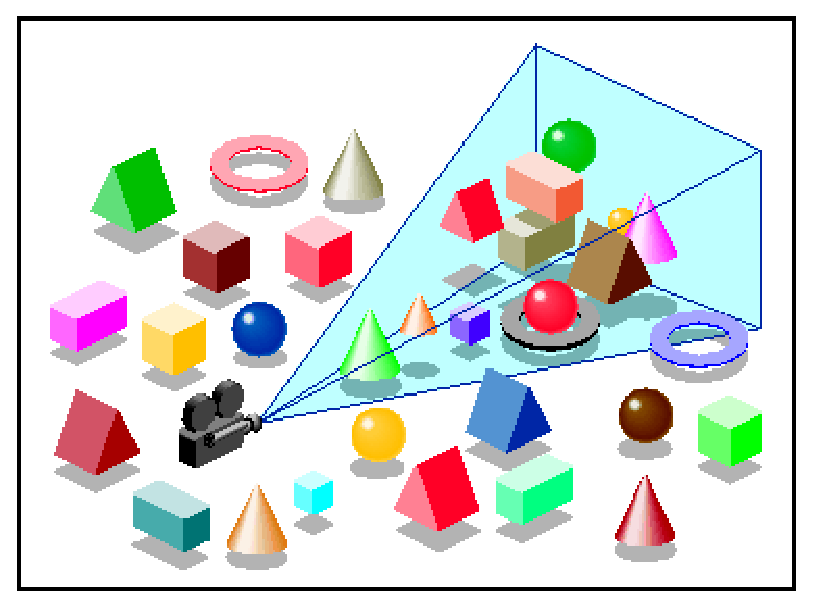
\epsfig{file=frustum1.eps, width=0.47\textwidth,clip=} &
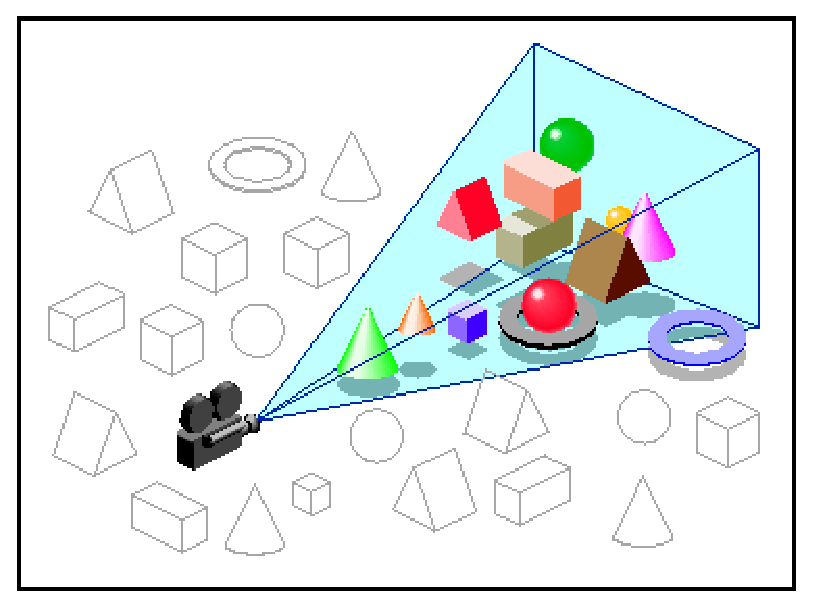
\epsfig{file=frustum2.eps, width=0.47\textwidth,clip=}
\end{longtable}
\vspace{-10pt}
\parbox{0.98\textwidth}{\captionof{figure}{Com o frustum culling os objetos que
est�o fora do campo de vis�o da c�mera n�o s�o enviados para o pipeline.}}
\end{center}

\subsection{Renderizador}

O renderizador da engine gr�fica utiliza um algoritmo de 3 fases:

\begin{itemize}
\item Atualiza��o dos n�s do grafo de cena
\item Processamento do grafo de cena
\item P�s-Processamento da imagem gerada pela fase de processamento
\end{itemize}

\vsection {Fase de atualiza��o}

Nessa fase, um \texttt{UpdaterVisitor} � utilizado para visitar e atualizar todos 
os n�s do grafo de cena. � a �nica fase n�o customiz�vel do algoritmo do renderizador.

\vsection {Fase de processamento do grafo de cena}

Nessa fase executa-se uma sequ�ncia de algoritmos definida pelo usu�rio da engine, a execu��o � equivalente ao c�digo:

%verificar se os argumentos est�o corretos
\begin{codigo}
std::vector<SceneProcessor*>::iterator it;
for(it = processors.begin(); it != processors.end(); it++){
   if(it->isActive()){
       it->process(gfx, renderer);
   }
}
\end{codigo}

Cada algoritmo deve implementar a interface \texttt{SceneProcessor}, 
que tem os seguintes m�todos:

\begin{itemize}
\item \texttt{bool isInitialized(GraphicAPI*)}: m�todo que indica se o algoritmo j� preparou todas as suas depend�ncias
\item \texttt{void initialize(GraphicAPI*, Renderer*)}: esse m�todo deve criar
todas as depend�ncias do m�todo \texttt{process}
\item \texttt{void process(GraphicAPI*, Renderer*)}: executa o algoritmo de processamento
\item \texttt{bool isActive()}: indica se o algoritmo deve ou n�o ser executado
\end{itemize}

\vsection{Fase de p�s-processamento}

Essa fase � semelhante � anterior, por�m o teste de profundidade do fragmento n�o � executado por padr�o, 
a implementa��o do algoritmo deve ativ�-lo manualmente.

A interface que deve ser implementada � a \texttt{ScenePostProcessor} que define m�todos com a mesma 
sem�ntica dos m�todos do \texttt{SceneProcessor}.

\subsubsection{Algoritmos de processamento de cena pr�-definidos}

% RenderPassProcessor esta passando da margem
O \texttt{RenderPassProcessor} �, atualmente, o �nico algoritmo de processamento
de cena padr�o da engine. Esse algoritmo utiliza \texttt{ColorPassVisitor} para
renderizar os n�s do grafo de cena.

\subsubsection{Algoritmos de p�s-processamento de cena pr�-definidos}
 
Atualmente existem 2 algoritmos de p�s-processamento padr�o implementados pelas
classes: \texttt{FramebufferImageProcessor} e \texttt{BlitToFramebuffer}.

O \texttt{FramebufferImageProcessor} � utilizado para fazer o p�s-processamento 
da imagem que estiver no buffer chamado \texttt{"color"} dentro do
\texttt{FramebufferObject} atual.
O algoritmo executado por esse objeto � descrito pelo c�digo abaixo:

\begin{codigo}
void FramebufferImageProcessor::process(GraphicAPI *gfx,
					Renderer *renderer) {
    std::map<std::string, Texture2D*> & renderables;
    renderables = renderer->getRenderables();
    
    Texture2D * auxBuffer = renderables["color_aux"];
    Texture2D * colorBuffer = renderables["color"];
    
    renderables["color"] = auxBuffer;
    renderables["color_aux"] = colorBuffer;
    
    FramebufferObject * fbo = renderer->getFramebufferObject();
    fbo->removeRenderable("color");
    fbo->addRenderable(auxBuffer, "color");
    fbo->update(gfx);
    
    UniformSampler2D* sampler = 
        dynamic_cast<UniformSampler2D*>(gfx->getUniformValue(
			UniformInfo("color", pbge::SAMPLER_2D)));
        				
    sampler->setValue(colorBuffer);
    renderer->renderScreenQuad(program.get());
}
\end{codigo}

O \texttt{BlitToFramebuffer} renderiza um ret�ngulo com as dimens�es 
da janela com a textura de nome \texttt{"color"} armazenada no renderizador. � utilizado 
para renderizar a imagem armazenada na textura \texttt{"color"} para o
framebuffer do sistema de janelas.

\subsubsection{Algoritmos de p�s-processamento customizados}

Foram desenvolvidos alguns algoritmos de p�s-processamento customizados como exemplo. 
Eles est�o dispon�veis na aplica��o de visualiza��o de campos tensoriais. A implementa��o 
de cada algoritmo se resume a um fragment shader utilizado para instanciar um 
\texttt{FramebufferImageProcessor}. Esse fragment shader recebe a posi��o do fragmento 
e uma textura contendo a imagem a ser renderizada.

\begin{itemize}
\item \textbf{Inversor de cores:} O algoritmo de invers�o de cores cria um vetor com 
os componentes \texttt{r,g,b}, calcula seu complemento e utiliza o resultado como 
a cor do fragmento:

\begin{codigo}
pbge::FramebufferImageProcessor * colorInversor() {
    return new pbge::FramebufferImageProcessor(
        "uniform sampler2D color;\n"
        "varying vec2 position;\n"
        "void main() {\n"
        "   vec3 color = (texture2D(color, position.xy)).rgb;\n"
        "   color = 1 - color;\n"
        "   gl_FragColor = vec4(color, 1);\n"
        "}\n"
    );
}
\end{codigo}
\item \textbf{Filtro de vermelho:} O filtro l� o componente veremelho da cor 
enviada pelo vertex shader e a utiliza no fragmento, sendo todos os outros 
componentes iguais a zero:

\begin{codigo}
pbge::FramebufferImageProcessor * chooseRed() {
    return new pbge::FramebufferImageProcessor(
        "uniform sampler2D color;\n"
        "varying vec2 position;\n"
        "void main() {\n"
        "   float r = (texture2D(color, position.xy)).r;\n"
        "   gl_FragColor = vec4(r, 0, 0, 1);\n"
        "}\n"
    );
}
\end{codigo}
\item \textbf{Lente senoidal:} A posi��o $(x_0, y_0)$ recebida � tal que 
$0 \leq x_0, y_0 \leq 1$. Ela � ent�o mapeada para $(x_1, y_1)$, onde 
$-1 \leq x_0, y_0 \leq 1$. � calculado ent�o o seno das componentes $x,y$ 
da posi��o multiplicadas por um fator que aumenta o efeito da lente. 
O resultado pertence ao intervalo $[-1,1]$, entretanto as coordenadas de 
textura est�o no intervalo $[0,1]$. Por esse motivo o seno � multiplicado 
por $0.5$ e somado a $0.5$ resultando em um valor no mesmo intervalo das 
coordenadas de textura. Esse valor � utilizado para ler uma posi��o com um 
pequeno deslocamento da posi��o do fragmento atual, com isso � gerada uma 
leve deforma��o que simula o efeito de uma lente:

\begin{codigo}
pbge::FramebufferImageProcessor * senoidalLens() {
    return new pbge::FramebufferImageProcessor(
        "varying vec2 position;\n"
        "uniform sampler2D color;\n"
        "void main(){\n"
        "   vec2 x = 2 * position - 1.0;\n"
        "   gl_FragColor = "
        "        texture2D(color, 0.5 + 0.5 * sin(1.5 * x));\n"
        "}"
    );
}
\end{codigo}
\end{itemize}

\subsection{Mecanismos da Engine}

\subsubsection{Mapeamento e gerenciamento dos estados}

Em placas de v�deo modernas, dispositivos altamente paralelos, as trocas de 
estado podem fazer com que o pipeline gr�fico tenha que ser esvaziado, o 
que pode causar um grande impacto no desempenho da aplica��o, por isso, � 
necess�rio evitar trocas de estado redundantes, minimizar trocas de estado 
e agrupar as trocas de estado.
% Esta repetindo trocas de estado muitas vezes

Na Pandora's Box, esse trabalho � delegado � classe \texttt{StateSet} e � duas
classes que controlam estados que podem ser desabilitados,
\texttt{BlendController} e \texttt{DepthController}. 

O \texttt{StateSet} � uma classe que controla a associa��o de objetos ao
contexto gr�fico. As modifica��es feitas atrav�s da \texttt{StateSet} s�o
sempre acumuladas e s� ocorrem quando o m�todo \texttt{updateState} � chamado.
O \texttt{updateState} primeiro atualiza as associa��es dos objetos gr�ficos ao
contexto e em seguida atualiza os par�metros do shader.

O \texttt{BlendController} controla a combina��o de fragmentos no framebuffer.
Ap�s ser gerado, se o fragmento n�o for descartado pelo teste de profundidade,
ele � enviado ao framebuffer e substitui o pixel correspondente, por�m utilizando o
\texttt{BlendController}, pode-se fazer com que o fragmento gerado se combine de
forma diferente com o pixel existente no framebuffer.

O \texttt{DepthController} configura o teste de profundidade, o teste de
visibilidade que � feito ap�s o fragment shader. Com esse controller � poss�vel, por exemplo
desabilitar o teste de profundidade.



\subsubsection{Desenho de modelos}

Existem 2 modos de se enviar v�rtices para serem processados pelo pipeline, 
atrav�s de \texttt{VertexBuffer} ou atrav�s de chamadas de fun��o obsoletas 
definidas pelo OpenGL, al�m disso, algumas vezes deseja-se que um mesmo modelo seja 
renderizado diversas vezes em um la�o (instanced draw). Para lidar com essas
situa��es, a Pandora's Box utiliza a classe \texttt{DrawController}.
% Instanced draw = geometry instancing? Se for precisa ver as ocorrencias no
% texto

O \texttt{DrawController} � respons�vel por enviar corretamente ao pipeline 
modelos definidos por inst�ncias de \texttt{VertexBuffer} (na engine tais 
modelos s�o inst�ncias de \texttt{VBOModel}) assim como inst�ncias de modelos 
que utilizam as fun��es obsoletas. Al�m de gerenciar a renderiza��o de um modelo, 
o \texttt{DrawController} � respons�vel por implementar o instanced draw.

Na Pandora's Box, instanced draw � implementado de forma nativa para \texttt{VBOModel}, 
ou seja, utilizando-se as fun��es espec�ficas do OpenGL que implementam a t�cnica, e 
de forma simulada se o modelo n�o for inst�ncia de VBOModel. 
A vers�o simulada da t�cnica � conhecida como pseudo-instancia��o. Em ambas as vers�es, 
uma vari�vel que indica qual � a inst�ncia do modelo que est� atualmente sendo renderizada. 
Essa t�cnica pode ser ilustrada pelo c�digo abaixo:
% O penultimo periodo desse paragrafo ta incompleto

\begin{codigo}
GraphicAPI * gfx = ...;
Model * model = ...;

// prepara o modelo para a renderiza��o
model->beforeRender(gfx);

for(int i = 0; i < number_of_instances; i++) {
    int instanceID = i;
    
    // renderiza a inst�ncia instanceID
    // a vari�vel instanceID fica dispon�vel no vertex shader
    model->render(gfx)
}

model->afterRender(gfx);
instanceID = 0;
\end{codigo}

\subsubsection{Passagem de par�metros para o GPUProgram}

A customiza��o do pipeline atrav�s de shaders gera grande flexibilidade, 
por�m essa customiza��o s� � interessante devido a possibilidade de passagem de diferentes par�metros para o shader.

Um programa do OpenGL pode receber tr�s tipos de par�metros:

% falar sobre built-in
\begin{itemize}
\item Uniformes: um valor que � constante para uma dada primitiva, 
  por exemplo, para um tri�ngulo, o processamento de seus tr�s v�rtices utilizam
  o mesmo valor de uniforme.
\item Uniformes built-in: s�o valores que se comportam como uniformes mas que
  s�o enviados automaticamente pelo OpenGL. As matrizes de transforma��o fazem
  parte dessa classe de valores.
\item Atributos: um valor que � constante para um v�rtice. Atributos s� podem ser 
  acessados dentro do \texttt{vertex shader}. No exemplo acima, cada um dos
v�rtices do tri�ngulo poderia ter um valor diferente para o atributo.
\end{itemize}

Dentro da Pandora's Box, o mecanismo de passagem de par�metros para o shader 
� implementado atrav�s das classes \texttt{UniformSet}, \texttt{UniformStack},
\texttt{GPUProgram}, \texttt{UniformValue} e \texttt{BuiltInUniformBinder} para
uniformes e da classe \texttt{AttribBinder} para atributos.

Como foi citado anteriormente, a �ltima etapa da atualiza��o de estados 
� a sincroniza��o dos par�metros do shader. Nessa fase, inicialmente, cada 
um dos \texttt{UniformInfo} gerados durante a compila��o do shader � utilizado 
para buscar um \texttt{UniformValue} dentro da \texttt{UniformStack}, o uniform 
value encontrado � ent�o associado ao programa atrav�s do mecanismo ilustrado 
no c�digo abaixo para o caso do GPUProgram implementado para OpenGL:

\begin{codigo}
void GLProgram::updateUniforms(GraphicAPI * gfx) {
    std::vector<UniformBindAndInfo>::iterator it;
    for(it = uniforms.begin(); it != uniforms.end(); it++) {
        UniformValue * value = gfx->searchUniform(it->getInfo());
        if(it->shouldUpdate(value)) {
            it->update(value);
            // associa o valor da uniforme ao shader
            value->bindValueOn(this, it->getInfo(), gfx);
        }
    }
}
\end{codigo}

% Talvez n�o citar todas as matrizes. Colocar referencias.

Ap�s essa etapa de associa��o de valores, as uniformes built-in s�o 
enviadas ao shader. O envio de built-ins � feito
atrav�s dos \texttt{BuiltInUniformBinder}, que s�o classes especializadas 
para cada um dos tipos de valor.

O mecanismo para o envio dos atributos � semelhante ao utilizada para enviar 
as uniformes \texttt{built-in}. Para cada um dos tipos de atributo definidos na
\texttt{enum} \texttt{Type} dentro da classe \texttt{pbge::VertexAttrib}
existe uma classe (\texttt{AttrBinder}) especializada em associar o atributo ao shader.
% Um dos texttt esta passando da linha

\subsection{Visualiza��o de campos tensoriais}

A aplica��o de visualiza��o de campos tensoriais � dividida em duas etapas:

\begin{itemize}
\item Compila��o do formato Analyze~\cite{Analyze} para o formato \texttt{.ctf}
(Compiled Tensor Field)
\item Apresenta��o do campo contido no arquivo \texttt{.ctg}
\end{itemize}

\subsubsection{O formato Analyze}

O formato Analyze � um formato de armazenamento de informa��es de imagens de resson�ncia magn�tica. A informa��o � dividida em dois arquivos: um cabe�alho (extens�o \texttt{.hdr}) com informa��es sobre o campo (dimens�es, ordena��o, identifica��o e hist�rico) e o arquivo de imagem (extens�o \texttt{.img}) contendo somente os valores da imagem (organizados conforme a descri��o do cabe�alho).

Para o desenvolvimento do leitor de arquivos Analyze foi feita a suposi��o de que os nomes dos arquivos (\texttt{.hdr} e \texttt{.img}) s�o iguais visando simplificar a utiliza��o e implementa��o.

\subsubsection{O formato Compiled Tensor Field (.ctf)}

O formato Compiled Tensor Field (\texttt{.ctf}) foi desenvolvido para armazenamento de informa��es sobre o campo tensorial a ser mostrado na aplica��o de visualiza��o de campos tensoriais. � um formato bin�rio que cont�m o n�mero de elips�ides (representa��o visual do tensor) no arquivo seguido por um conjunto de matrizes de transforma��o linear. Cada matriz ser� aplicada a uma esfera para obter um elips�ide na posi��o correta no campo. Por esse motivo ela cont�m uma escala (proporcional aos autovalores do tensor aplicados nos eixos cartesianos), uma rota��o (dos eixos cartesianos para os eixos definidos pelos autovetores do tensor) e uma transla��o (para posicionar o elips�ide corretamente no campo).

Na etapa de compila��o a imagem de resson�ncia magn�tica � lida e os tensores
armazenados em um vetor. Nessa etapa todos os tensores nulos s�o ignorados. Um
tensor $A_{3
\times 3}$ � considerado nulo quando o m�dulo de todas as suas entradas �
maior do que um dado $\varepsilon > 0$. Ou seja, $A$ � nulo quando a seguinte express�o � v�lida
para $i, j \in \mathbb{Z}$, $1 \leq i, j \leq 3$:

% Ficou melhor explicado assim?
\vspace{10pt}
\hspace{10pt}
\begin{math}
|A_{i,j}| < \varepsilon
\end{math}
\vspace{10pt}

S�o ent�o calculados os autovalores e autovetores de todos os tensores n�o nulos, geradas as matrizes de transforma��o linear que levam uma esfera centralizada na origem para um elips�ide na posi��o correta no campo e armazenadas em um vetor. 

Como tais matrizes s�o matrizes de transforma��o homog�nea, a �ltima linha sempre ser� $(0,0,0,1)$. Assim � poss�vel ocultar tais dados e enviar outras informa��es em seu lugar (� necess�rio substituir os valores dessa linha para realizar quaisquer opera��es com a matriz). Nessa linha s�o armazenados os valores das equa��es (\ref{af}), (\ref{linearCase}), (\ref{planarCase}) e (\ref{sphericalCase}) (definidas na p�gina \pageref{af}) que ser�o utilizados como diferentes pol�ticas de escolha de n�vel de transpar�ncia (alfa) e cor dos elips�ides.

As matrizes s�o ent�o reorganizadas em blocos de proximidade para otimizar a utiliza��o pela aplica��o de visualiza��o. O vetor de matrizes reordenado � finalmente escrito no arquivo, al�m das informa��es iniciais sobre o campo.

\subsubsection{Apresenta��o do campo compilado}

O arquivo \texttt{.ctf} � lido e cada bloco de matrizes � enviado como \texttt{uniform} para o \texttt{shader} que as aplica a esferas. A pol�tica de transpar�ncia (alfa) dos elips�ides � escolhida pelo usu�rio, sendo o valor de alfa algum dos quatro resultados das equa��es de anisotropia fracionada. A cor aplicada a cada elips�ide � calculada a partir do valor de alfa em uma rampa de cores tamb�m definida pelo usu�rio.

\begin{center}
\begin{longtable}{cc}
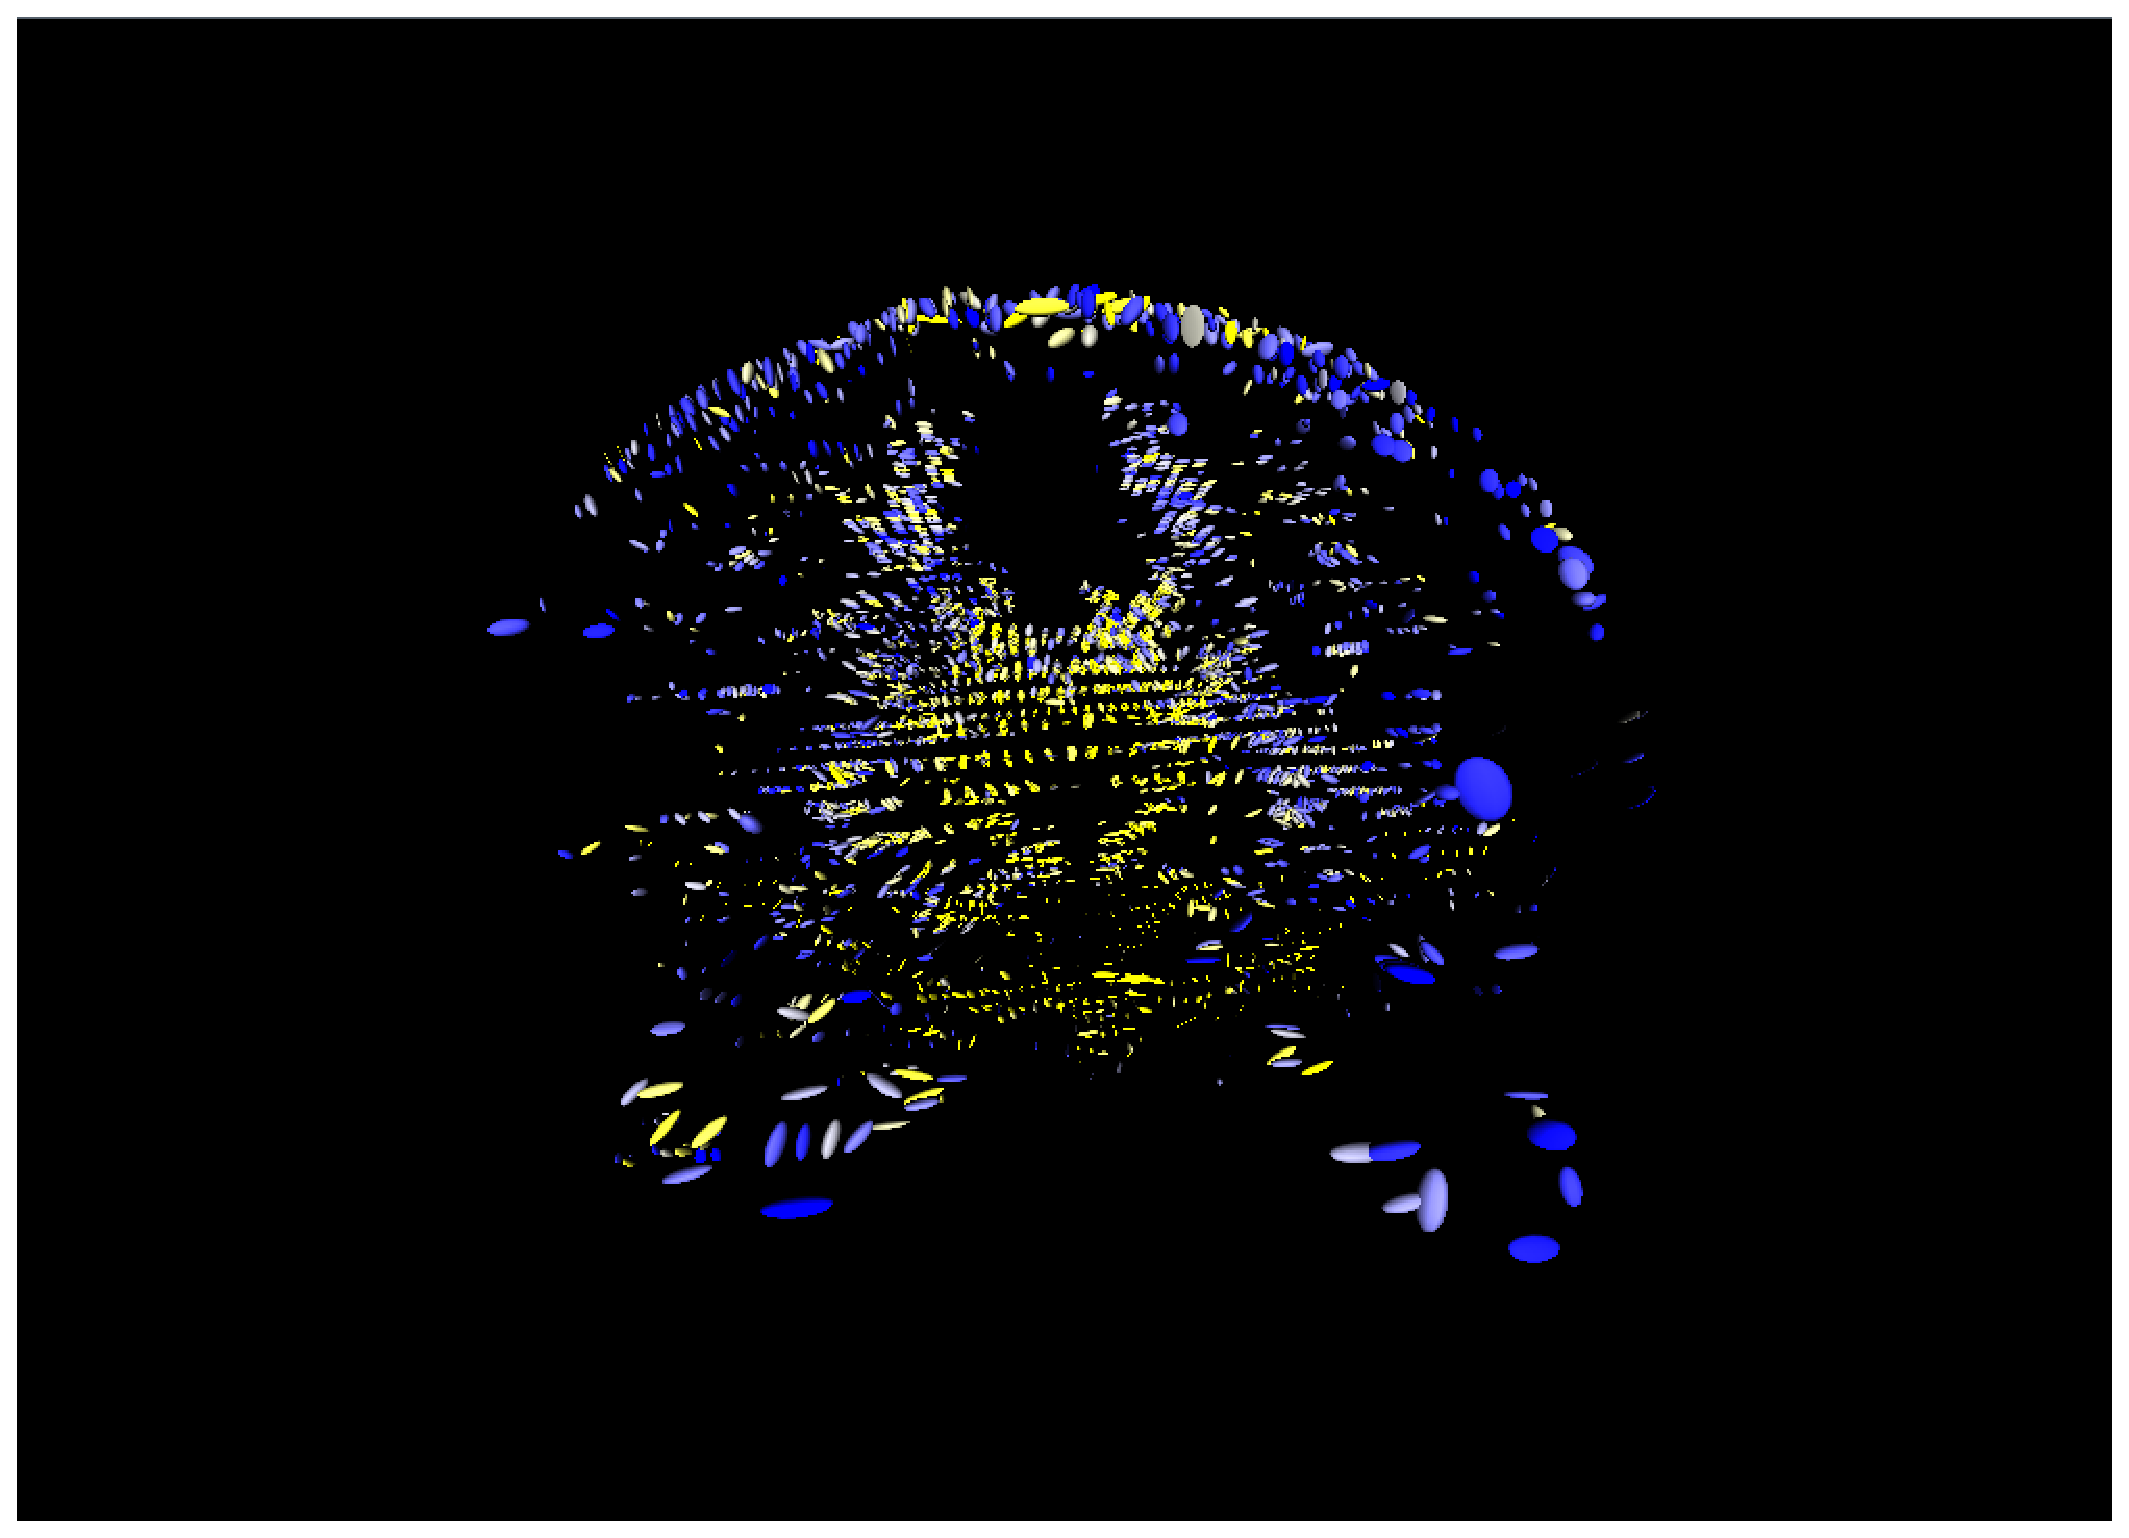
\epsfig{file=cerebro1.eps, width=0.47\textwidth,clip=} &
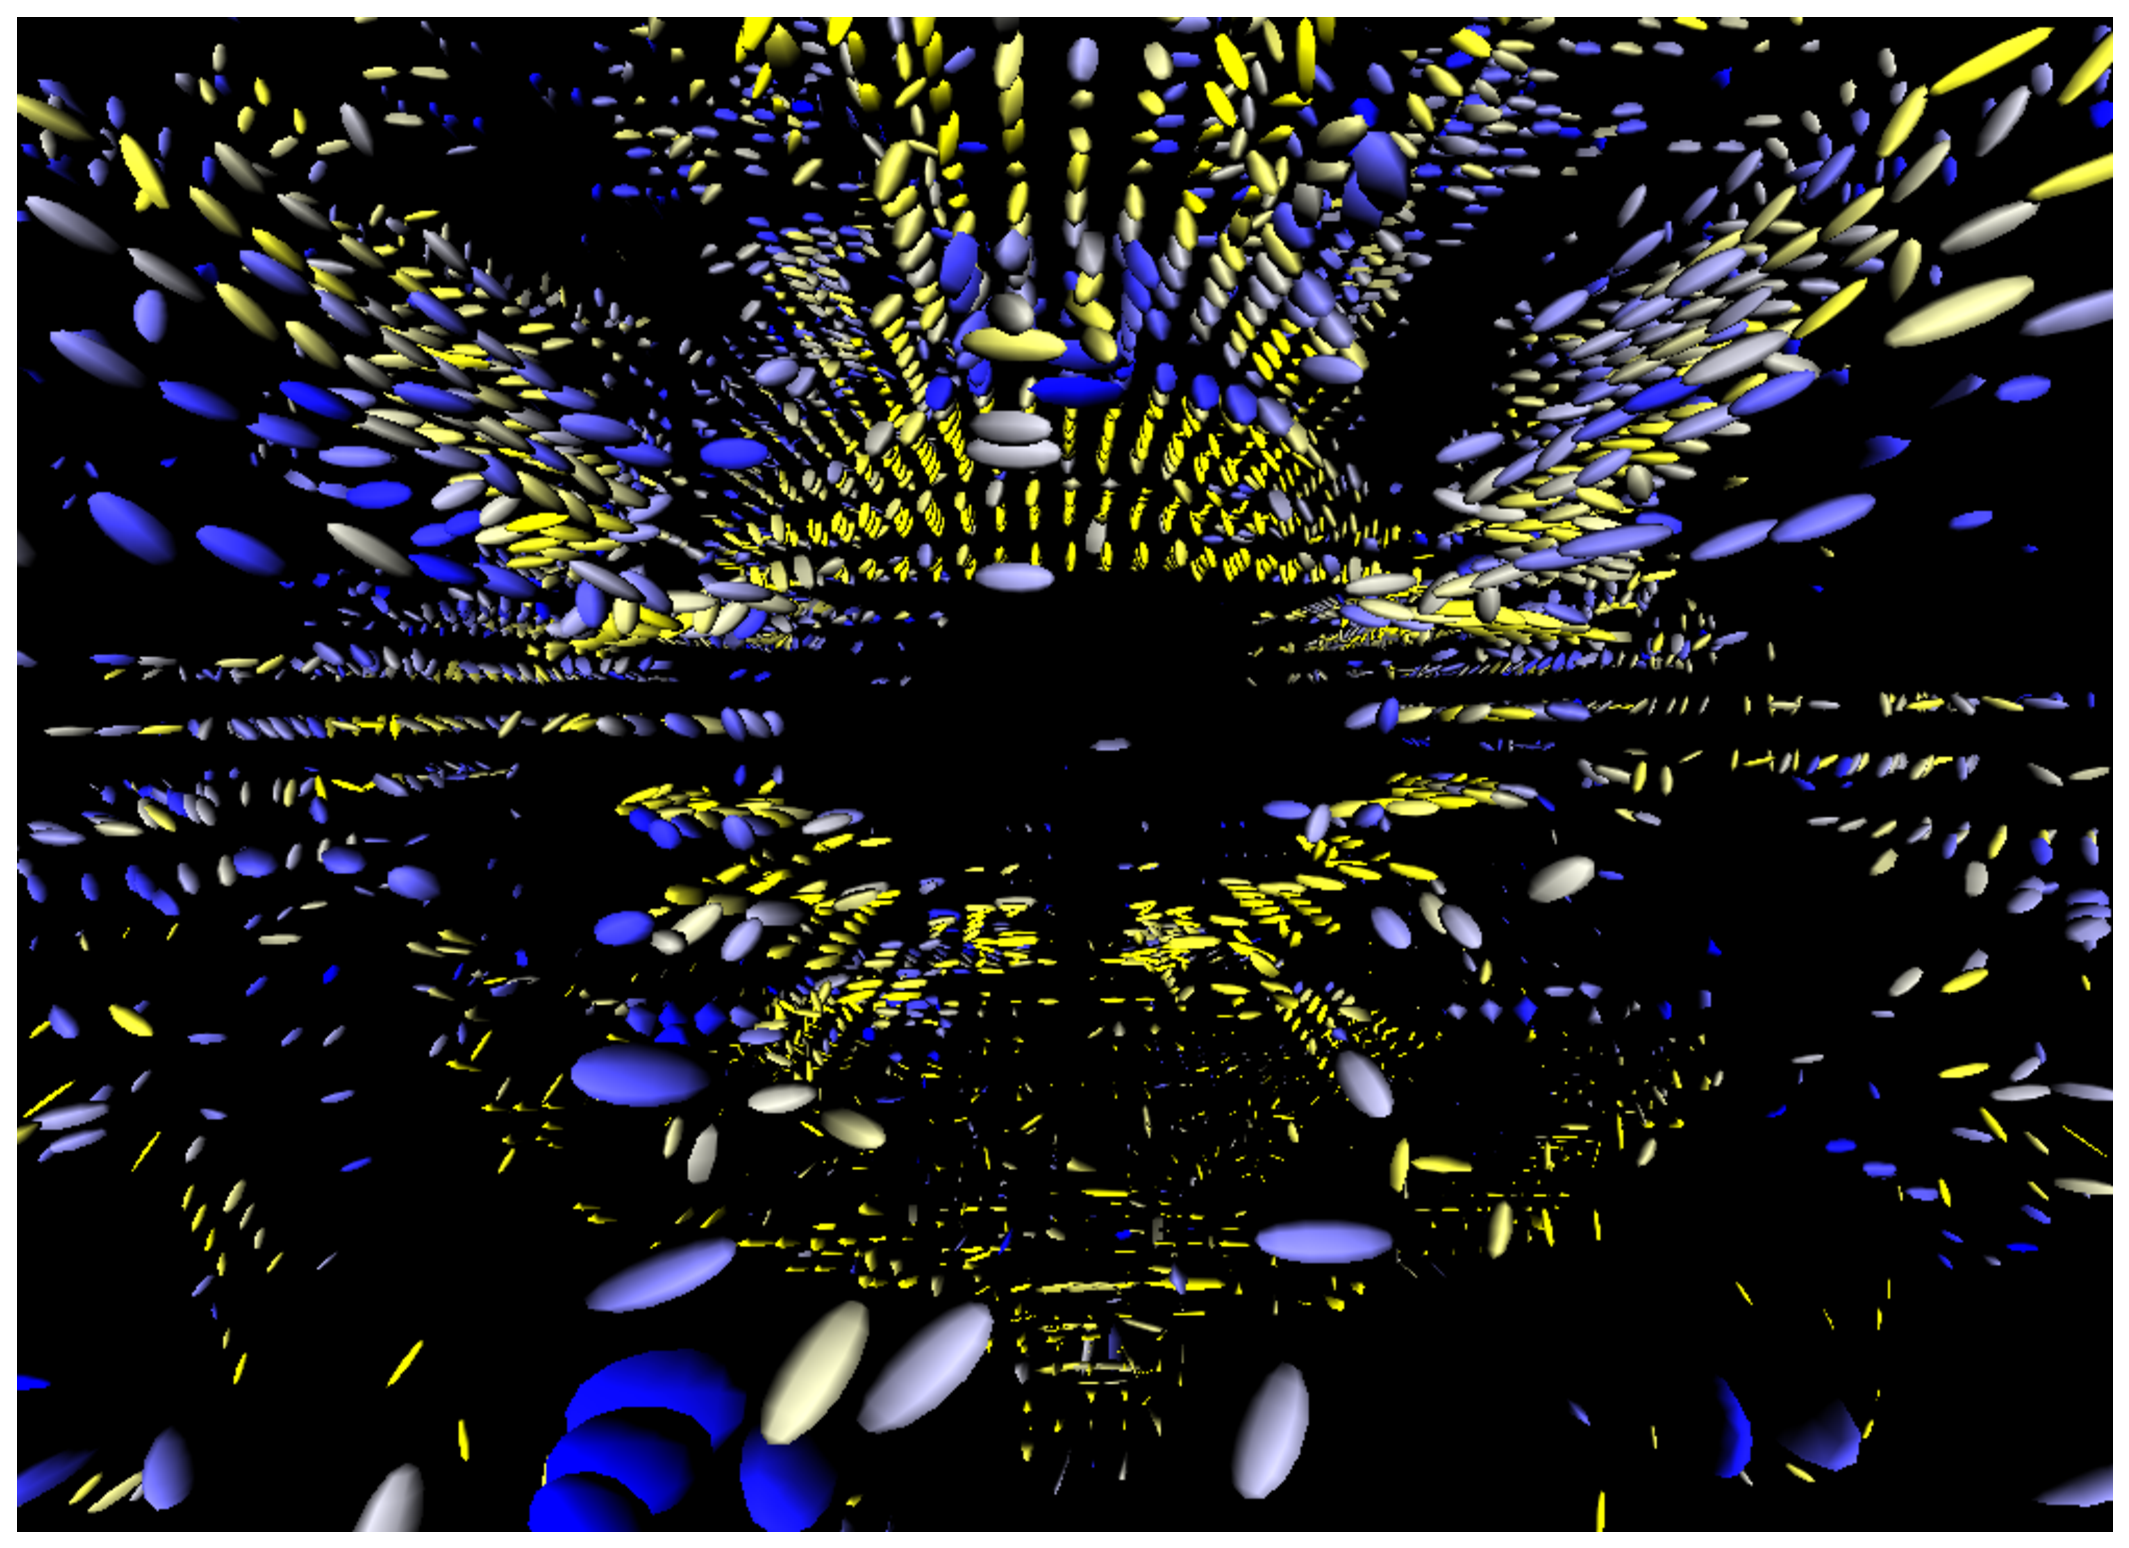
\epsfig{file=cerebro2.eps, width=0.47\textwidth,clip=}
\end{longtable}
\vspace{-15pt}
\parbox{0.98\textwidth}{\captionof{figure}{Imagens da
visualiza��o do campo tensorial de um c�rebro humano. As cores s�o aplicadas a partir do valor de
anisotropia fracionada em uma rampa de cores que varia do azul (menor
anisotropia) para o amarelo (maior anisotropia).}}
\end{center}

Para a transla��o e rota��o do campo foram implementados um \texttt{KeyboardEventHandler} e um \texttt{MouseEventHandler} respectivamente que atualizam os n�s de transforma��o.

\subsection{T�cnicas aplicadas}

\subsubsection{Depth Peeling}
No campo tensorial em diversos casos existem elips�ides sobrepostos. Para observar alguns tipos de estrutura � interessante que tais elips�ides possuam algum n�vel de transpar�ncia. Para isso � necess�rio simular a transpar�ncia atrav�s de combina��es de cores sobrepostas. Existem t�cnicas~\cite{alphasorting} que dependem dos objetos serem renderizados dos mais distantes para os mais pr�ximos da c�mera, entretanto no caso do campo esse tipo de processo se torna muito lento devido � grande quantidade de objetos a serem ordenados antes de cada renderiza��o. Por esse motivo � necess�rio algum algoritmo independente da ordem de renderiza��o.

Depth peeling~\cite{everitt} � uma t�cnica iterativa que consiste de remo��es de camadas pr�ximas a cada itera��o. Inicialmente a cena � renderizada normalmente armazenando o color buffer e o 
 buffer em buffers auxiliares. A cada nova itera��o todos os fragmentos com profundidade menor ou igual � profundidade armazenada no depth buffer auxiliar s�o descartados. Um novo depth buffer auxiliar � gerado a partir das profundidades dos fragmentos restantes, que s�o ent�o renderizados e o resultado (color buffer) � acumulado no color buffer auxiliar.

Para a realiza��o da t�cnica completa s�o necess�rias $N$ itera��es, onde $N$ �
o n�mero m�ximo de fragmentos sobrepostos na cena. Entretanto na aplica��o foi
fixado um n�mero de itera��es para diminuir a complexidade da t�cnica.

Na aplica��o de exemplo o depth peeling foi implementado como um processador de cena sendo que a cada itera��o o grafo de cena � percorrido uma vez.

As imagens abaixo exemplificam essa t�cnica com duas esferas acompanhadas do resultado da itera��o.

\begin{wrapfigure}{l}{\textwidth}
\vspace{-20pt}
\begin{center}
\subfigure[Primeira itera��o]{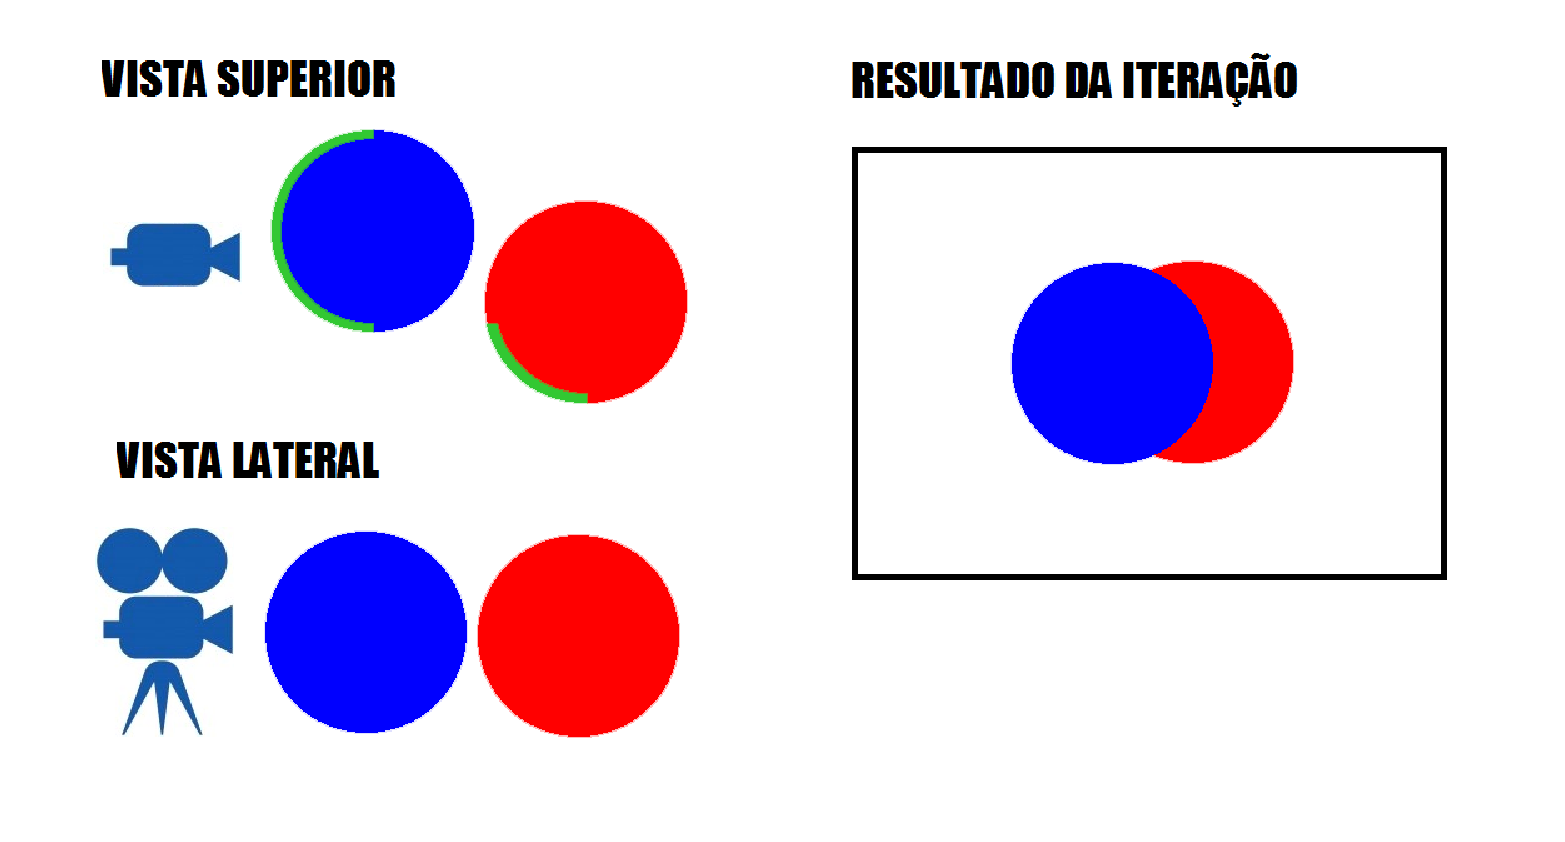
\includegraphics[width=0.49\textwidth]{depthpeeling1}}
\subfigure[Segunda itera��o]{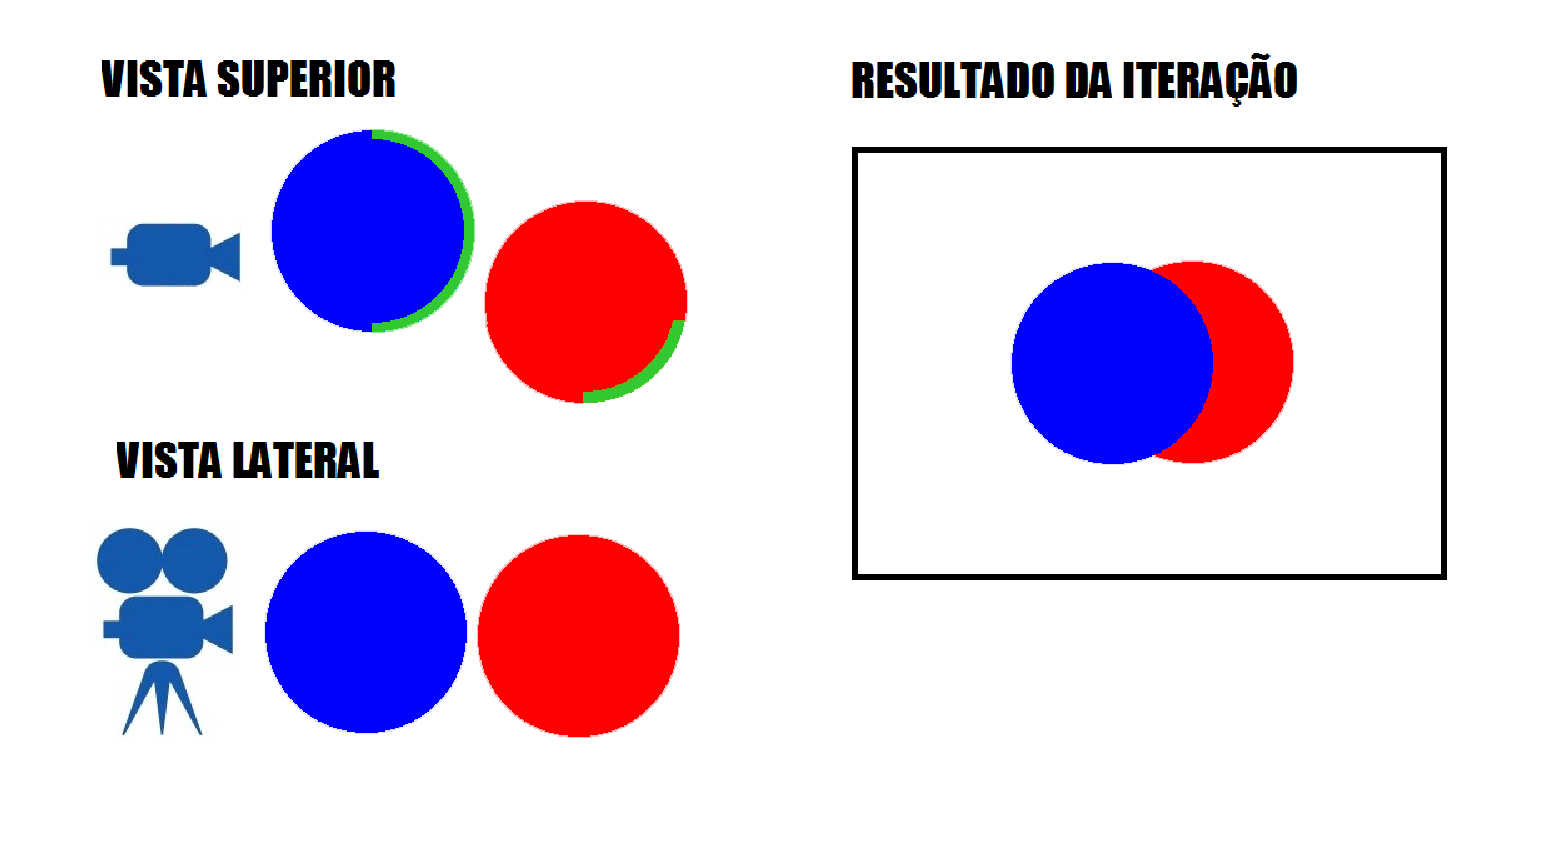
\includegraphics[width=0.49\textwidth]{depthpeeling2}}
\subfigure[Terceira itera��o]{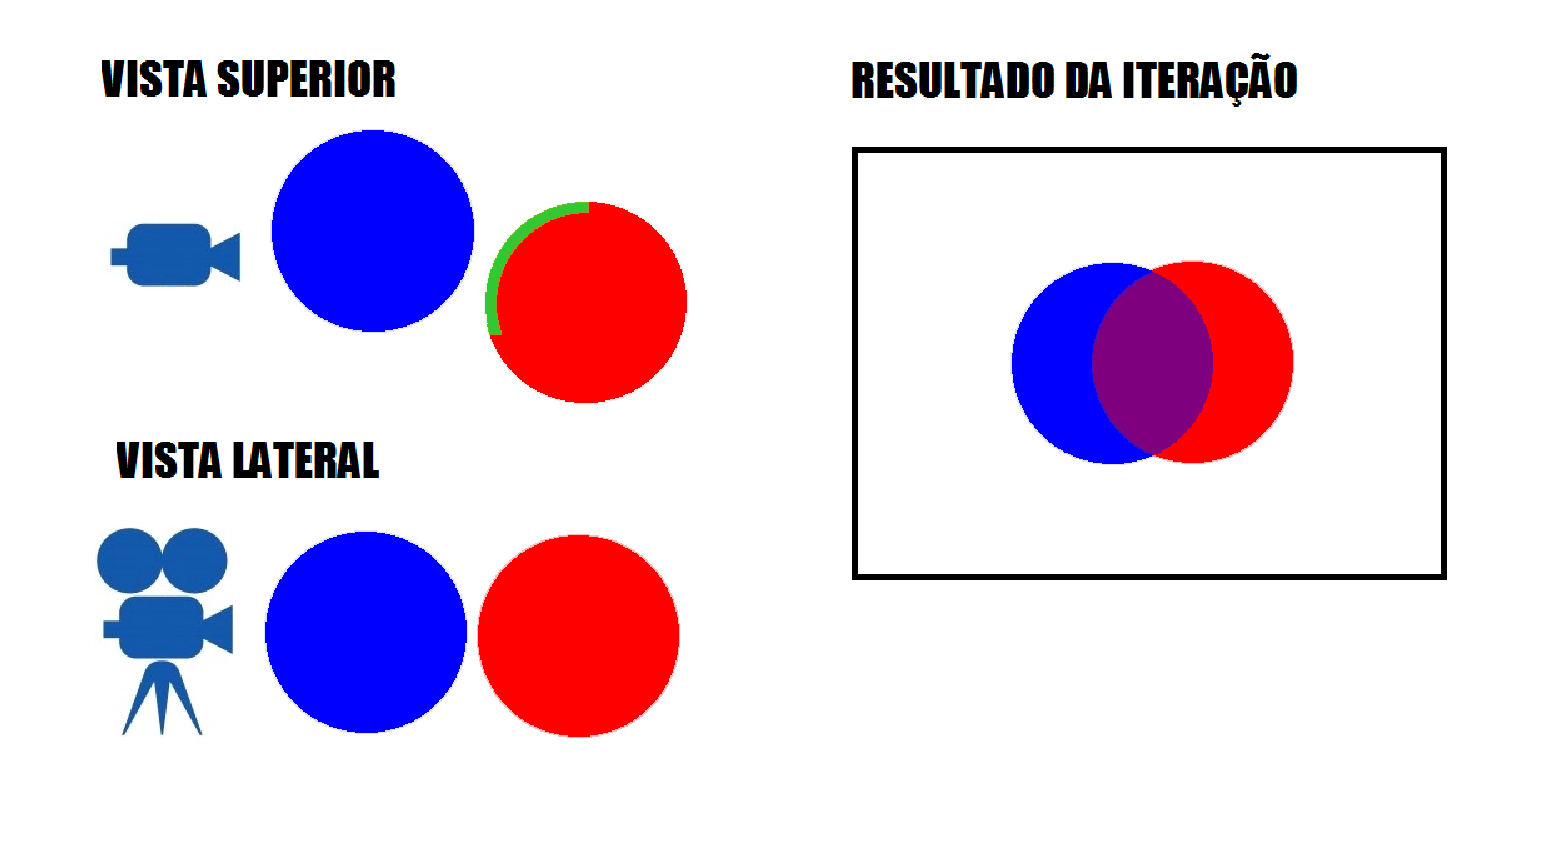
\includegraphics[width=0.49\textwidth]{depthpeeling3}}
\end{center}
\vspace{-20pt}
\caption{Em cada itera��o do depth peeling � desconsiderada uma camada de
fragmentos. A imagem � combinada ao resultado anterior considerando-se a
opacidade de cada pixel.}
\vspace{-10pt}
\end{wrapfigure}


\section{Resultados e produtos obtidos}

O c�digo do Pandora's Box Graphics Engine, assim como da aplica��o de visualiza��o de campos tensoriais e outros exemplos pode ser encontrado no seguinte endere�o:

\url{https://github.com/victorkendy/PandoraBox}

\subsection{Compilador de campos tensoriais}
A aplica��o de compila��o de campos tensoriais pode ser executada atrav�s da linha de comando com os seguintes argumentos opcionais:

\begin{verbatim}
field_compiler.exe [ARQUIVO DO CAMPO] [ARQUIVO CTF]
\end{verbatim}

Caso o programa seja executado sem nenhum argumento o usu�rio deve escolher entre as op��es 1 e 2 (campo de uma dupla h�lice sint�tica e de um c�rebro humano respectivamente). A op��o \texttt{ARQUIVO DO CAMPO} deve indicar o nome de um arquivo .img sem a extens�o (sup�e-se que o arquivo .hdr tenha o mesmo nome), ou seja, suponha que existam os arquivos \texttt{campo.hdr} e \texttt{campo.img}, ent�o o argumento deve ser \texttt{campo}. O �ltimo argumento deve ser o nome do arquivo .ctf a ser criado, por exemplo \texttt{campo.ctf}.


\section{Conclus�es}
Para o desenvolvimento de aplica��es de computa��o gr�fica s�o necess�rias diversas t�cnicas de otimiza��o e organiza��o das informa��es. A Pandora's Box Graphics Engine tem por objetivo disponibilizar uma interface simples para utiliza��o de algumas dessas t�cnicas:

\begin{itemize}
\item As cenas s�o representadas por grafos de cena nos quais � poss�vel utilizar os n�s j� definidos na engine ou criar novos tipos para implementar outras t�cnicas
\item Uma cena pode ser renderizada atrav�s dos processadores de cena adicionados ao renderizador sendo poss�vel tamb�m criar novos processadores (que percorram o grafo executando m�todos espec�ficos de n�s customizados, por exemplo)
\item A utiliza��o de shaders se resume a escrever o c�digo e associ�-lo a algum n� do grafo (a compila��o e o bind s�o gerenciados pela engine)
\item Texturas s�o gerenciadas pela engine, cabendo ao usu�rio carreg�-las e associ�-las a n�s do grafo de cena
\end{itemize}

Com o aux�lio da Pandora's Box foi poss�vel desenvolver algumas aplica��es de exemplo, incluindo o visualizador de campos tensoriais de imagens de resson�ncia magn�tica sens�veis � difus�o. Essa aplica��o exigiu a utiliza��o de diversas t�cnicas de otimiza��o para ser poss�vel a visualiza��o de campos com grandes quantidades de tensores em tempo real. 

Nessa aplica��o � poss�vel restringir a informa��o apresentada retirando-se tensores dependendo do seu n�vel de anisotropia e observar estruturas internas. Ainda existem diversas melhorias a serem feitas tanto na engine quanto na aplica��es de exemplo, entretanto j� � poss�vel utiliz�-las da maneira como foram propostas. Com as aplica��es desenvolvidas a Pandora's Box Graphics Engine se mostrou capaz de lidar com grandes quantidades de informa��o, al�m de ser facilmente customiz�vel para diferentes finalidades.

% Comentario sobre possiveis trabalhos futuros
% Falta escrever mais um pouco e fechar tudo


\nocite{*}
\newpage \bibliographystyle{plain}
\bibliography{bibliografia_monografia}

\end{document}
